\documentclass[12pt]{article}
\usepackage{graphicx} %for embedding images
\usepackage{url} %for proper url entries
\usepackage{hyperref}
\usepackage{float}
%\usepackage{caption}
%\usepackage{subcaption}
\usepackage{pdfpages}
%
\begin{document}
\renewcommand{\thefootnote}{\arabic{footnote}}

%include other pages
\begin{titlepage}

\begin{center}

\vfill

% Title
\LARGE \textbf {John Deere XUV Gator 850D}\\
\LARGE \textbf {Robot Documentation}\\[0.5in]

\small \textbf{Justin Poh, Claire Diehl, Ryan Eggert, Caleb Kissel} \\
\small \textbf{Academic Year 2015 - 2016}

\vspace{.1in}
Under the guidance of\\
{\textbf{Professor David Barrett}}\\[0.2in]

\vspace{.1in}
Supported by:\\
{\textbf{Student Academic Grant (SAG) \\ Franklin W. Olin College of Engineering}}\\[0.2in]

\vfill

% Bottom of the page

\includegraphics[scale=0.17]{Logos.jpg}
\Large{Intelligent Vehicles Laboratory}\\
\normalsize
\textsc{Franklin W. Olin College of Engineering}\\
Needham, Massachusetts \\


\end{center}

\end{titlepage}


\tableofcontents

\newpage

\listoffigures

\newpage

\listoftables

\newpage
\chapter{Preface}

Hello Reader! \\ \\
%
\noindent My name is Justin Poh and I am (was) a senior at Olin College who graduated in May 2016. If you're reading this document, you must be working on the John Deere Gator XUV vehicle. Well, you're joining a unique group of individuals who have been working on this vehicle starting with the 2009 - 2010 SCOPE team. \\ \\
%
This document is meant to be a manual for how to run, use and work on the vehicle at the point that we left it. We also intended for this document to serve as something that can be continuously updated by subsequent teams of students in an easy and efficient manner. As such, in addition to the PDF and printed copies of this document, the original files are stored in a github repository at \url{https://github.com/olinrobotics/GatorResearch_Documentation}. Since everything was written in Latex, downloading any Latex editor should allow anyone to modify this document and update it as the state of the vehicle changes. I hope you find this document useful as you work on the vehicle and good luck! \\ \\
%
Cheers,\\ \\
%
Justin Poh\\
Ground Vehicle Lead, Olin Intelligent Vehicles Laboratory\\
Class of 2016
\newpage
\section{The Mechanical System}

\subsection{The Original Components}
Most of the mechanical components on board the vehicle were installed by the SCOPE team that first worked on the vehicle in 2009 - 2010. As such, this section begins by including the original pages from the 2009 - 2010 SCOPE team report describing the mechanical system. \\ \\
%
Today, this mechanical system remains largely the same except for the following changes:

\begin{enumerate}
\item The monitor mentioned in the original SCOPE team report is the Nortec SUN-1710-P daylight-visible monitor. The current monitor on the vehicle is a standard Acer monitor
\end{enumerate}

\newpage

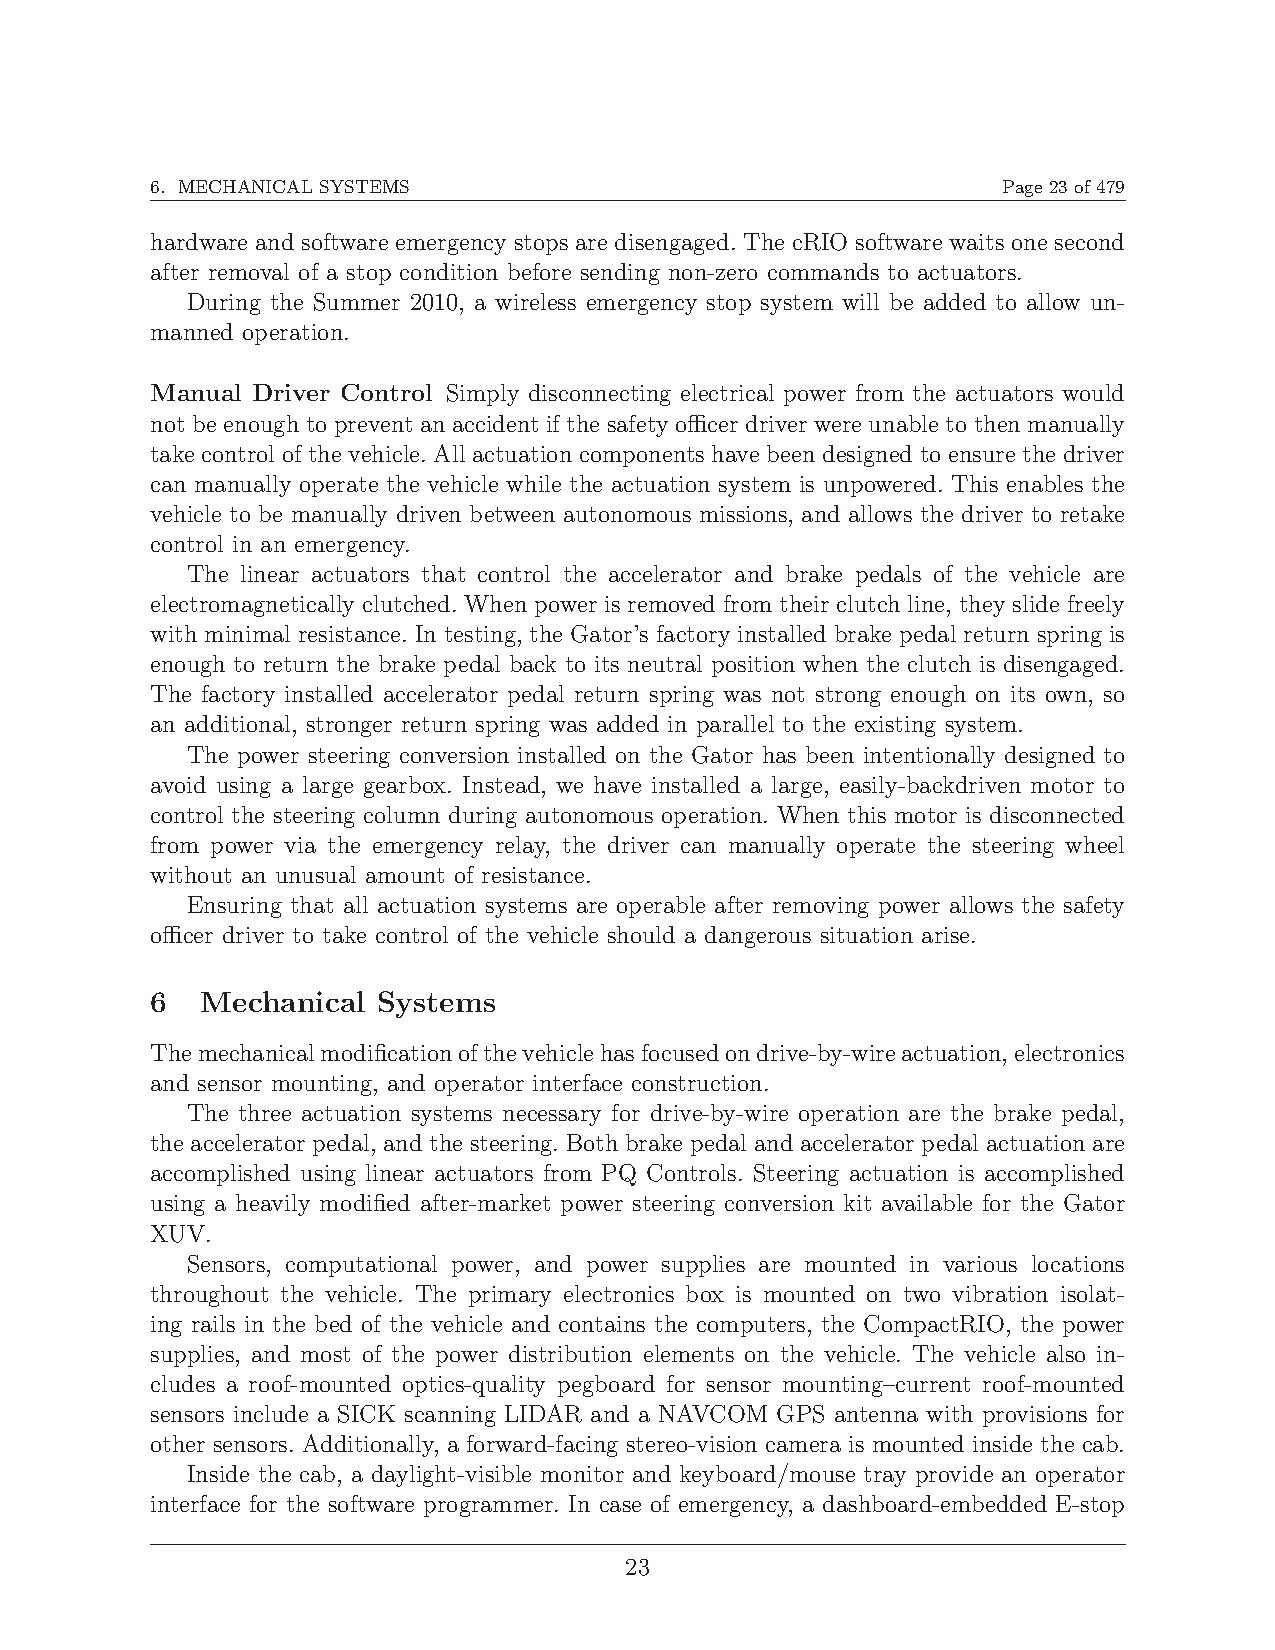
\includepdf[scale=0.9, pages=-, clip, trim=0mm 20mm 0mm 35mm, pagecommand={}]{MechSystem.pdf}

\newpage

\subsection{Additional Mechanical Components}
\newpage
\section{The Electrical System}

The electrical system consists of two parts: the power distribution system and signals. Each will be discussed in the following sections. Wiring diagrams are provided in Appendix.

\subsection{The Power Distribution System}

\subsubsection{Power Supplies}
Power to the entire system comes from the 3-prong plug running through the PVC pipe fixtures on the driver's left side of the electronics box.

\begin{figure}[h!]
\centering
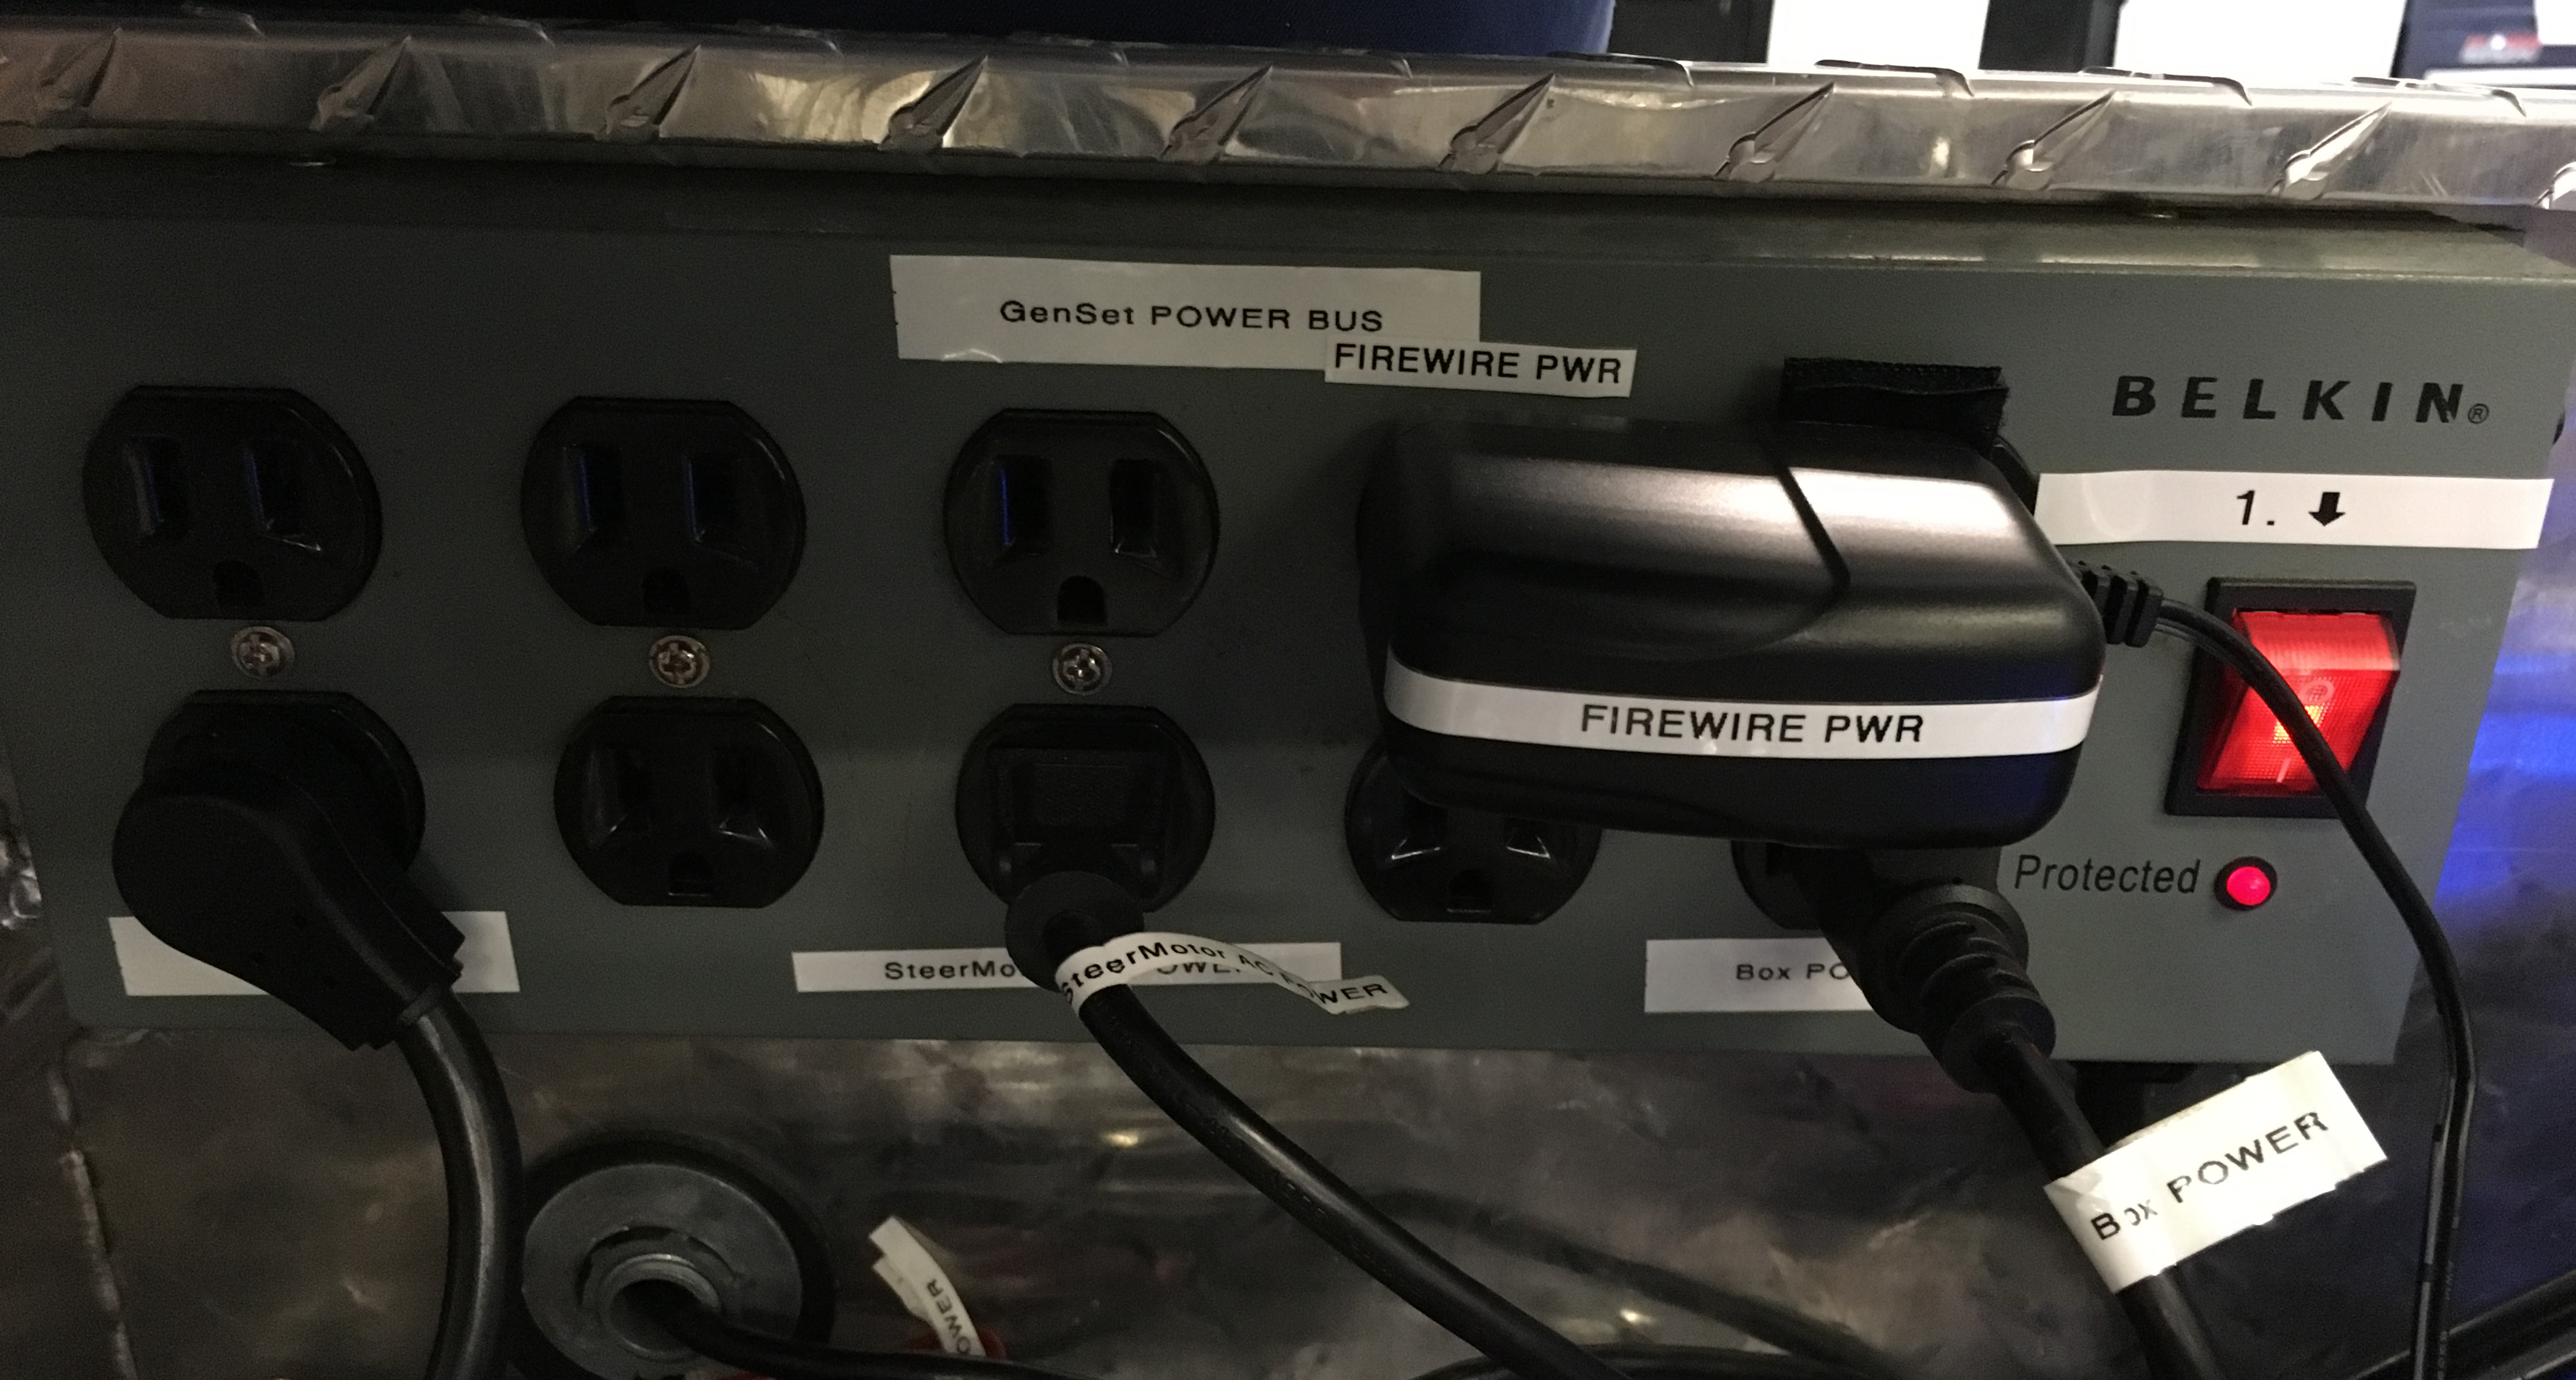
\includegraphics[scale=.1]{Photos/PowerStrip.jpg}
\caption{The power strip on the side of the electronics box}
\label{fig:powerstrip}
\end{figure} 

 \noindent The 3-prong plug attached to the power strip plugs into building power when the vehicle is in the Large Project Building and supplies power to the power strip mounted on the wall of the electronics box on the driver's left side. Alternatively, during operation, the 3-prong plug is plugged into a Honda EU2000i generator that should be mounted in the back of the vehicle:\\ \\
%
 Power to the rest of the system is then drawn from that power strip. The devices plugged into that power strip are shown in the diagram below:\\ \\

\begin{figure}[h!]
\centering
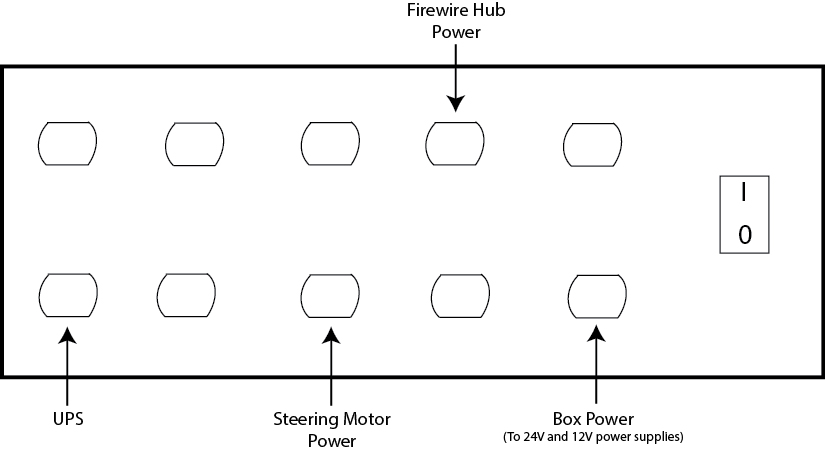
\includegraphics[scale=.6]{Photos/PowerStrip_Drawing.jpg}
\caption{Drawing of devices plugged into the power strip}
\label{fig:powerstripdrawing}
\end{figure} 

\noindent The entire system has 3 voltages that powers everything: 5 volts, 12 volts and 24 volts:
\begin{enumerate}
\item A Meanwell HRP-600-24 converts 120V AC power from the power strip to 24V DC power
\item A Meanwell HRP-300-12 converts 120V AC power from the power strip to 12V DC power
\item A Meanwell SB-15B-05 converts 24V DC power from the 24V DC power supply to 5V DC power
\end{enumerate}
%
The 24V and 12V power supplies are located on the lower deck of the electronics enclosure and the 5V power supply is located on the upper deck.

\newpage 

\subsubsection{Fuses}
There are 4 main fuse blocks used on the vehicle to distribute power via fuses to all electronic devices on board:
\begin{enumerate}
\item 1 Blue Sea Systems fuse block (C24) handles all 24V power distribution
\item 2 Blue Sea Systems fuse blocks (C12 and M12) handle all 12V power distribution
\item 1 linear fuse block handles all 5V power distribution 
\end{enumerate}
%
From the lower deck, three main power busses run to the upper deck: two 24V busses and one 12V bus. One 24V bus runs to the C24 fuse block and the other 24V bus runs to the 5V power supply that converts 24V DC power to 5V DC power. The 12V bus runs to the M12 fuse block. The C12 fuse block is powered from one of the outputs on the M12 fuse block.
%
\subsubsection{24V Power Distribution}

\begin{minipage}{0.6\textwidth}
Five outputs on the C24 fuse block are used:\\
\begin{enumerate}
\item Signal to a 24V sensing probe
\item LIDAR power
\item LIDAR power
\item Navcomm GPS power
\item Safety light power
\end{enumerate}
\end{minipage} \hfill
\begin{minipage}{0.5\textwidth}
\begin{figure}[H]
\centering
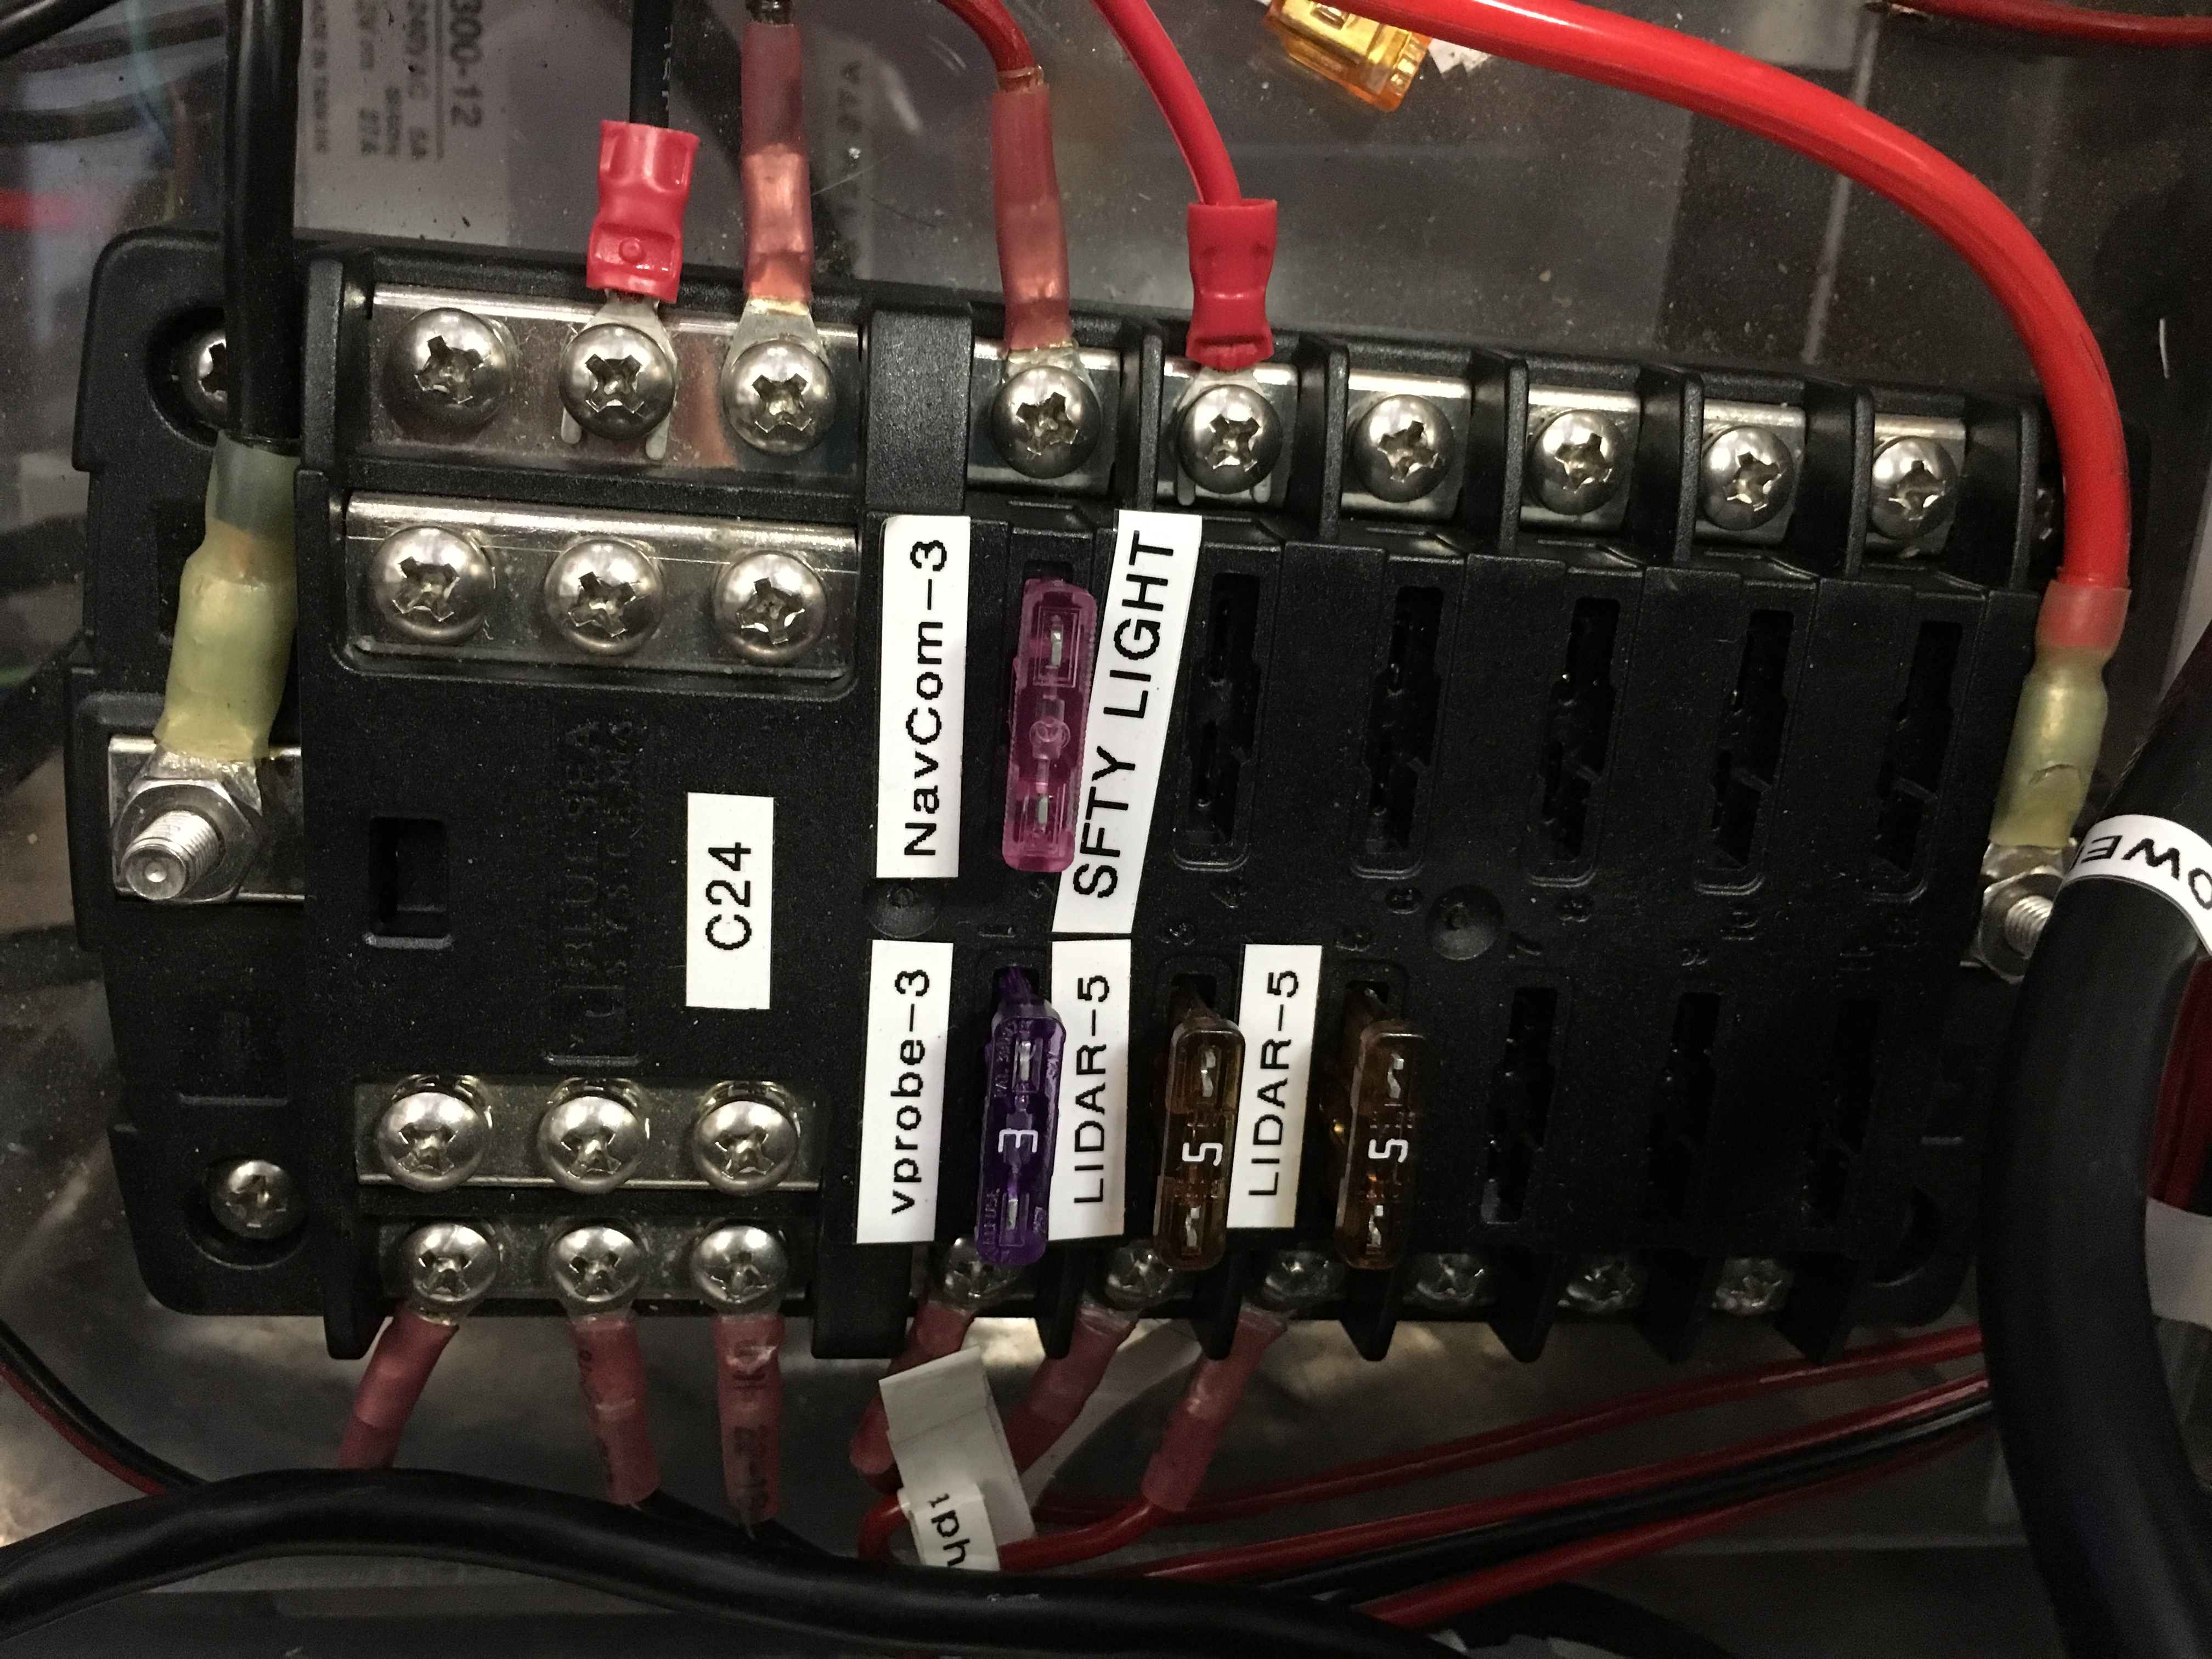
\includegraphics[scale=.05, angle=-90]{Photos/C24.jpg}
\caption{\label{fig:C24} C24 Fuse Block}
\end{figure}
\end{minipage}

\bigskip

\noindent  Except for the signal to the 24V sensing probe, all of the other 4 lines run to the appropriate equipment outside the electronics box. The signal to the 24V sensing probe runs to the voltage sense project box (discussed in a later subsection).

\newpage

\subsubsection{12V Power Distribution (C12 Fuse Block)}

\begin{minipage}{0.6\textwidth}
Five outputs on the C12 fuse block are used:
\begin{enumerate}
\item Power for the cab fans
\item Signal to a 12V sensing probe
\item INS power
\item Power for ethernet switch
\item E-Stop 12V power
\end{enumerate}
\end{minipage} \hfill
\begin{minipage}{0.5\textwidth}
\begin{figure}[H]
\centering
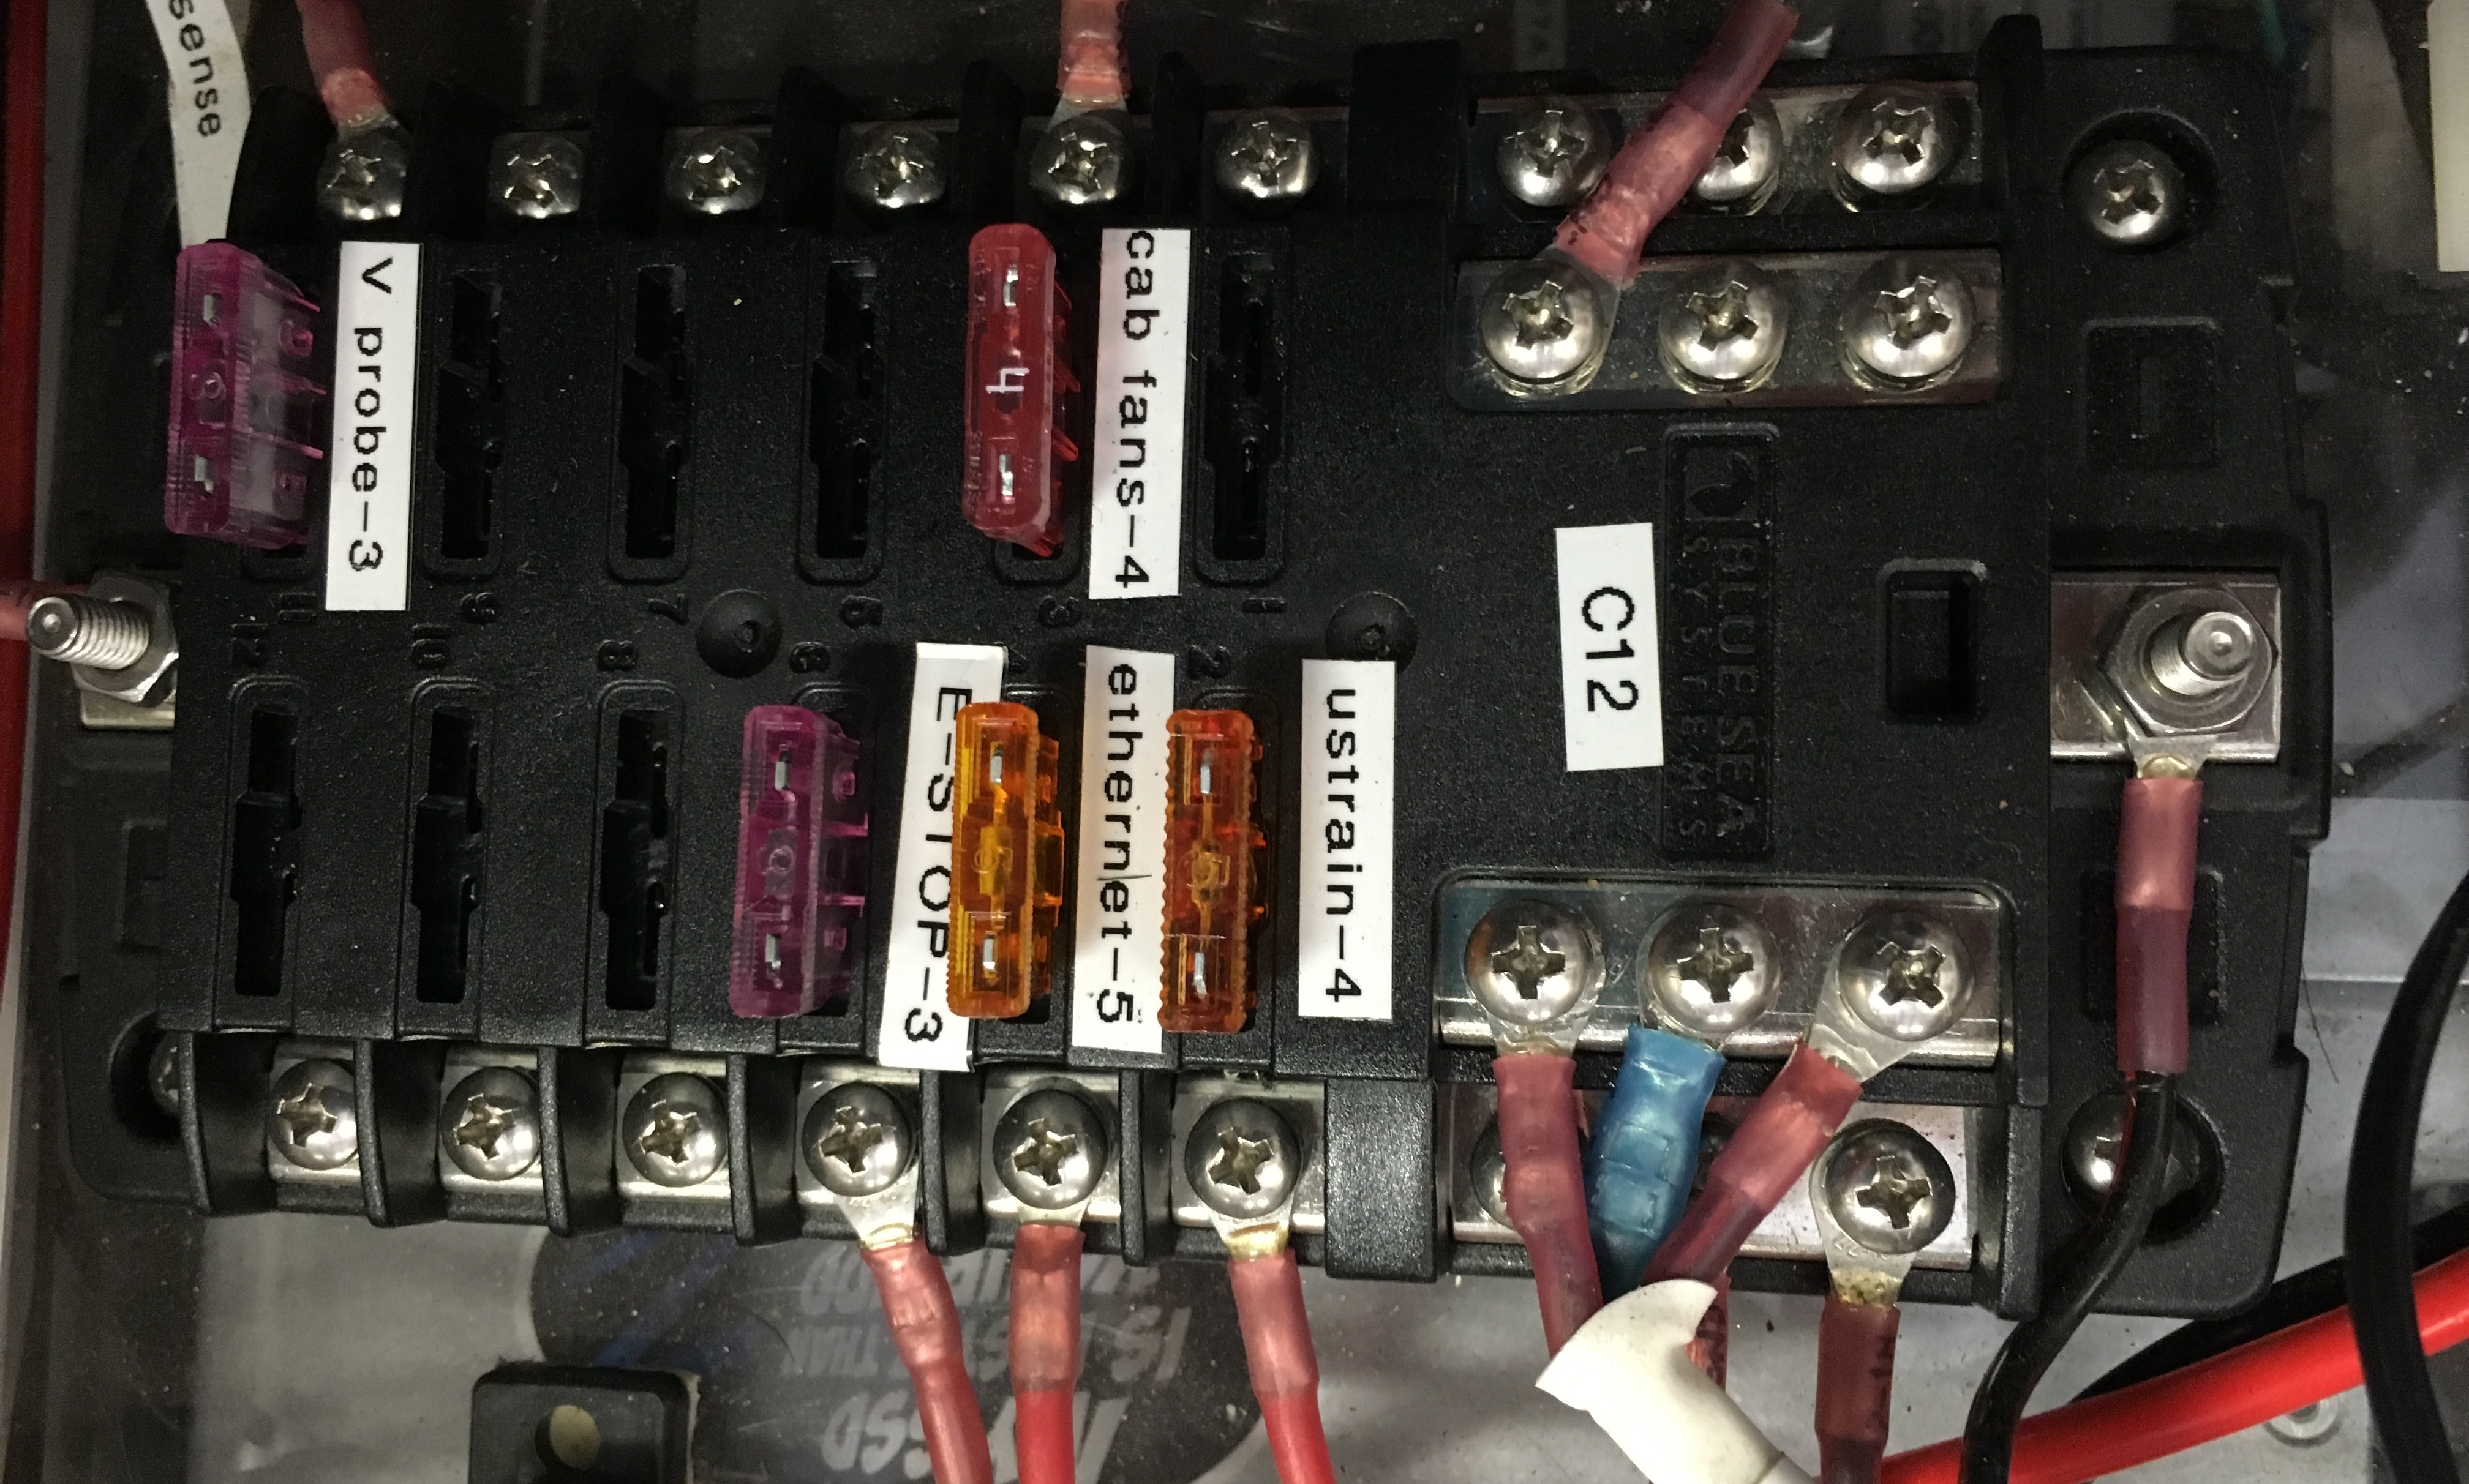
\includegraphics[scale=.06, angle=90]{Photos/C12.jpg}
\caption{\label{fig:C12} C12 Fuse Block}
\end{figure}
\end{minipage}

\bigskip

\noindent Power for the cab fans and INS power run to the appropriate equipment outside the electronics box. The signal to the 12V sensing probe runs to the voltage sense project box (discussed in a later subsection) and power to the ethernet switch runs to the netgear ethernet switch on the back corner of the electronics box on the driver's right side of the vehicle. The E-Stop 12V power is utilized by the E-Stop system, which will be discussed in a later section.

\subsubsection{12V Power Distribution (M12 Fuse Block)}

\begin{minipage}{0.6\textwidth}
All six outputs on the M12 fuse block are used:
\begin{enumerate}
\item Right tilt unit motor power
\item Power to the C12 fuse block
\item Power to the linear actuators
\item Left tilt unit motor power
\item Box fan power
\item Box fan power
\end{enumerate}
\end{minipage} \hfill
\begin{minipage}{0.5\textwidth}
\begin{figure}[H]
\centering
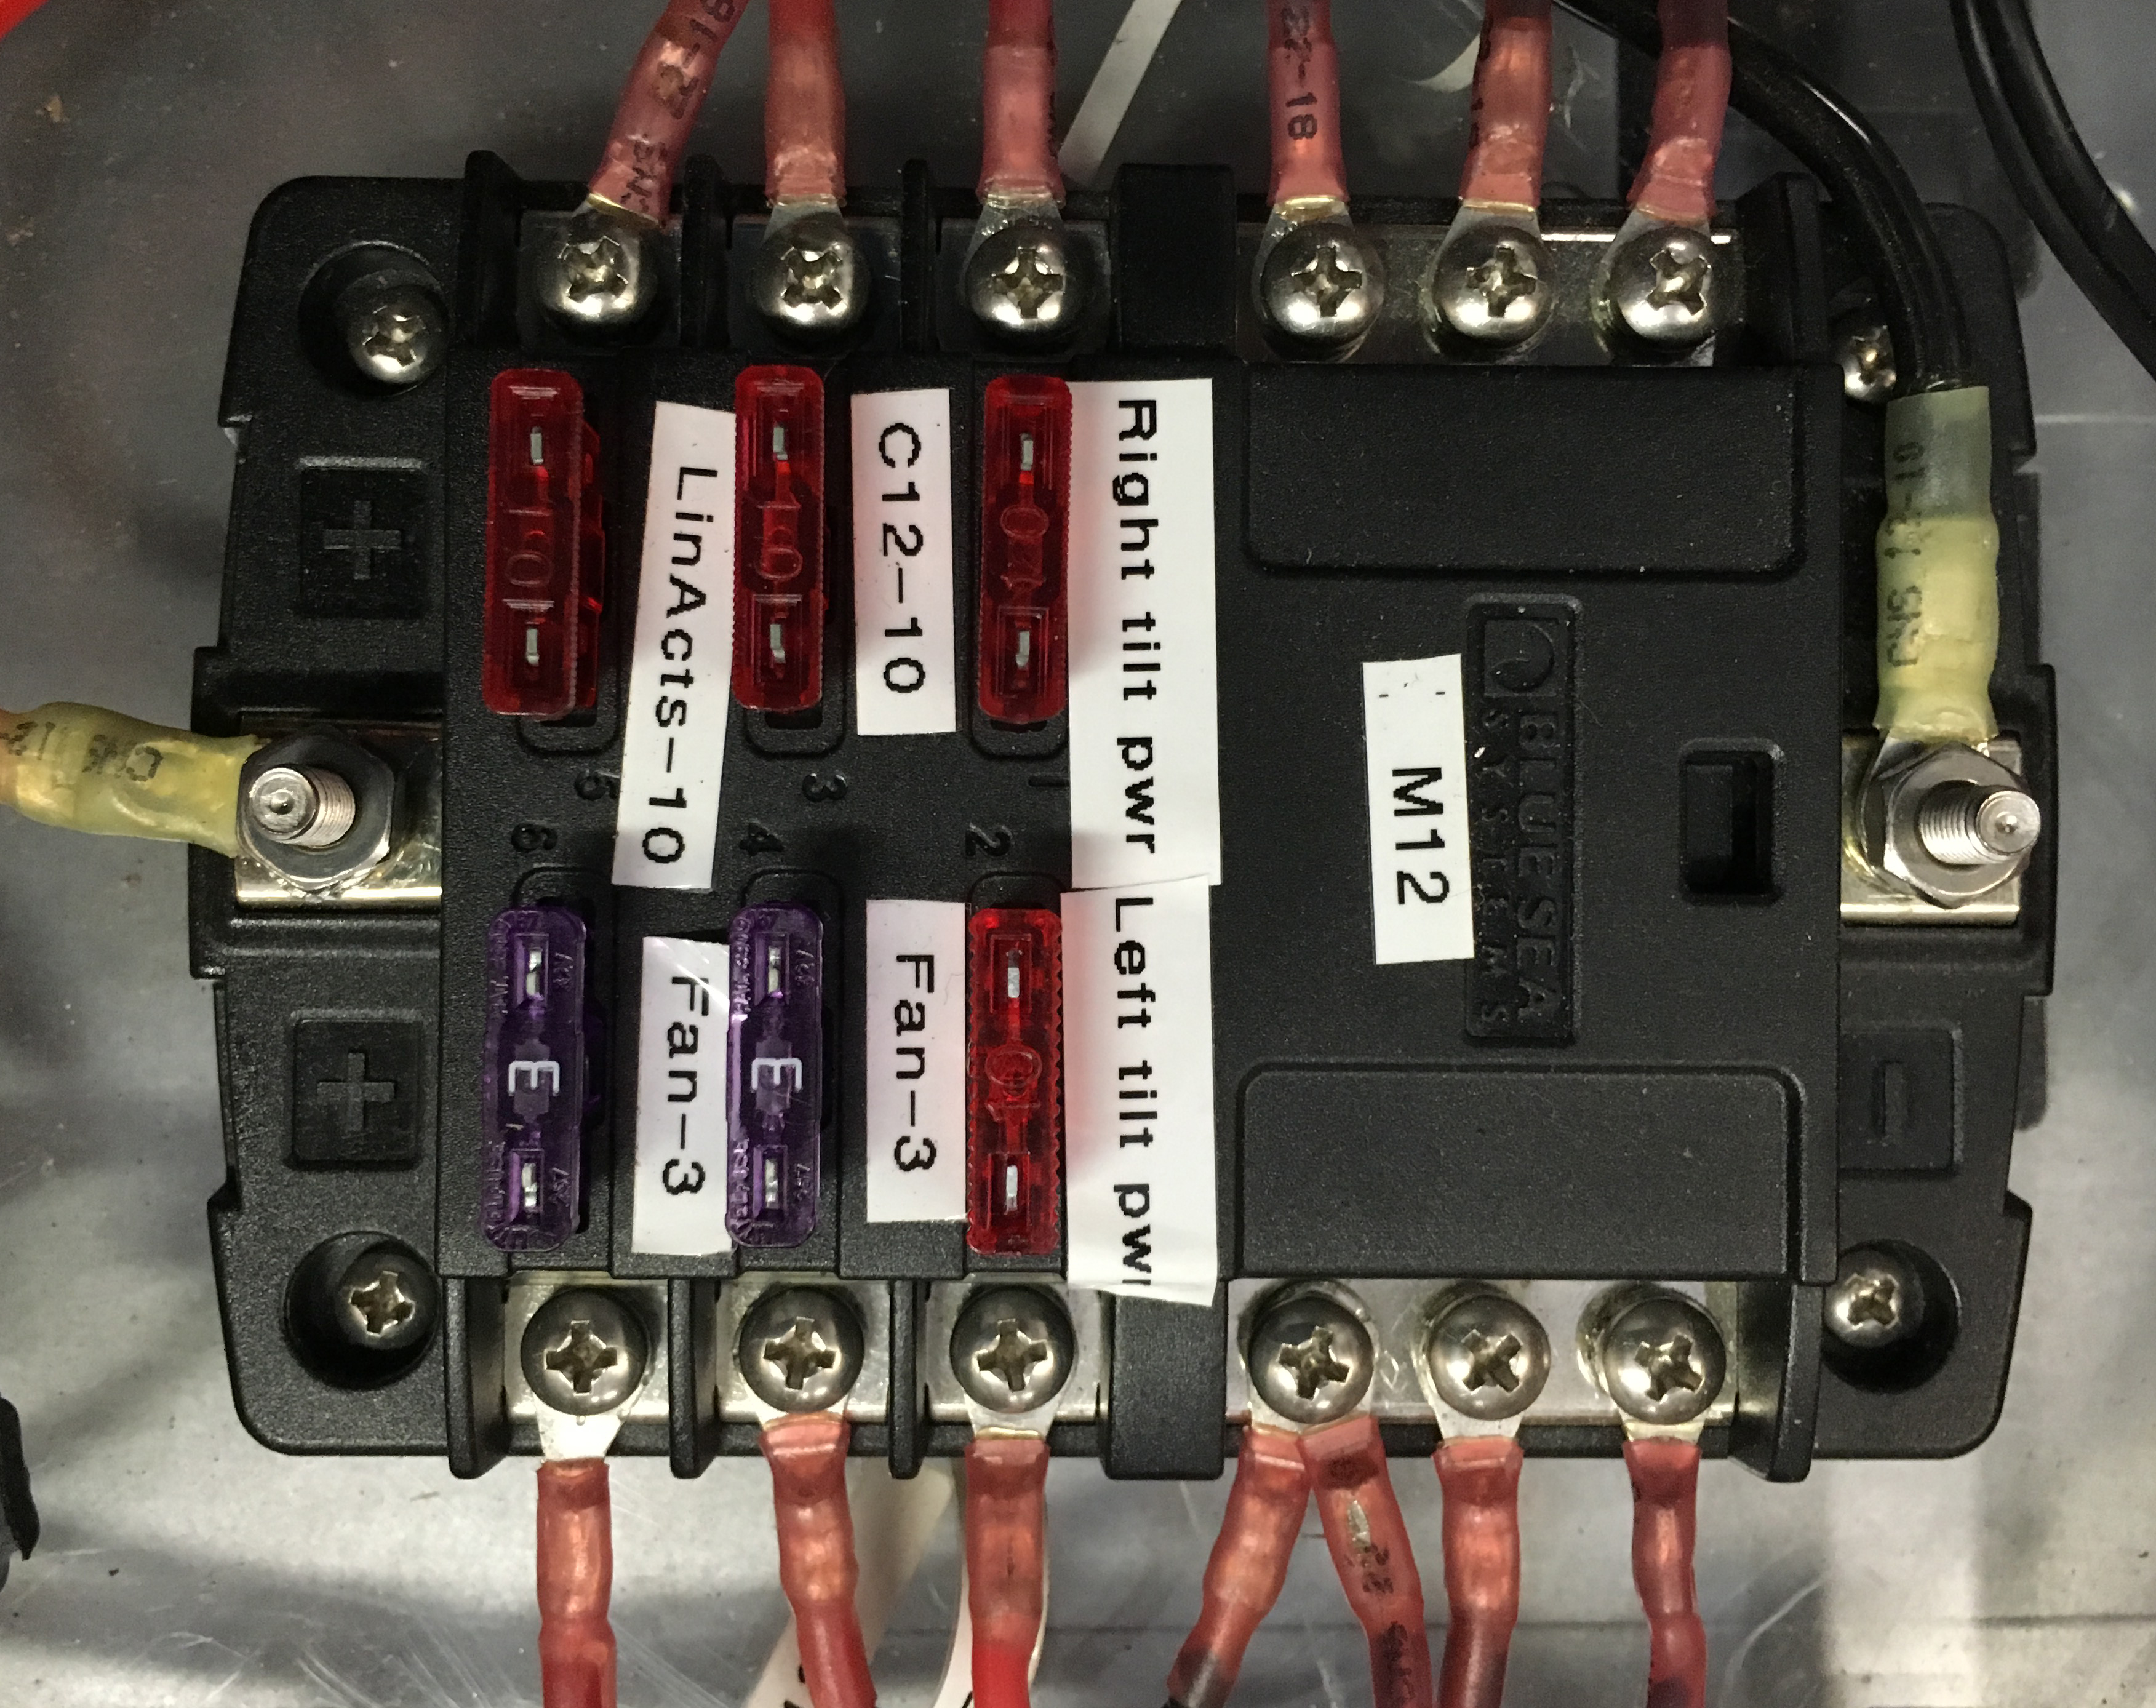
\includegraphics[scale=.06, angle=90]{Photos/M12.jpg}
\caption{\label{fig:M12} M12 Fuse Block}
\end{figure}
\end{minipage}

\bigskip

\noindent The power to the C12 fuse block is obtained from the appropriate port on the M12 fuse block. The power to each of the fans mounted to the front of the electronics box that cools the electronics box is also obtained from 2 of the outputs. Power to the right and left tilt units is also drawn from the M12 fuse block outputs and power then runs to the appropriate equipment outside the electronics box. Finally, the power for the linear actuators runs to an E-Stop relay first, then connected to two fuse terminals on the linear fuse block (discussed on the next page)

\subsubsection{Linear Fuse Block (Various Power Distribution)}

\begin{minipage}{0.6\textwidth}
The four lines on the linear fuse block are:
\begin{enumerate}
\item Fuse for motor power coming from the steering motor amplifier headed to the steering motor
\item Fuse for the 5V DC power output from the 5V DC power supply headed to the 5V DC power terminal strip
\item Two fuses to distribute 12V power from the E-Stop relay to the gas and brake linear actuators
\end{enumerate}
\end{minipage} \hfill
\begin{minipage}{0.5\textwidth}
\begin{figure}[H]
\centering
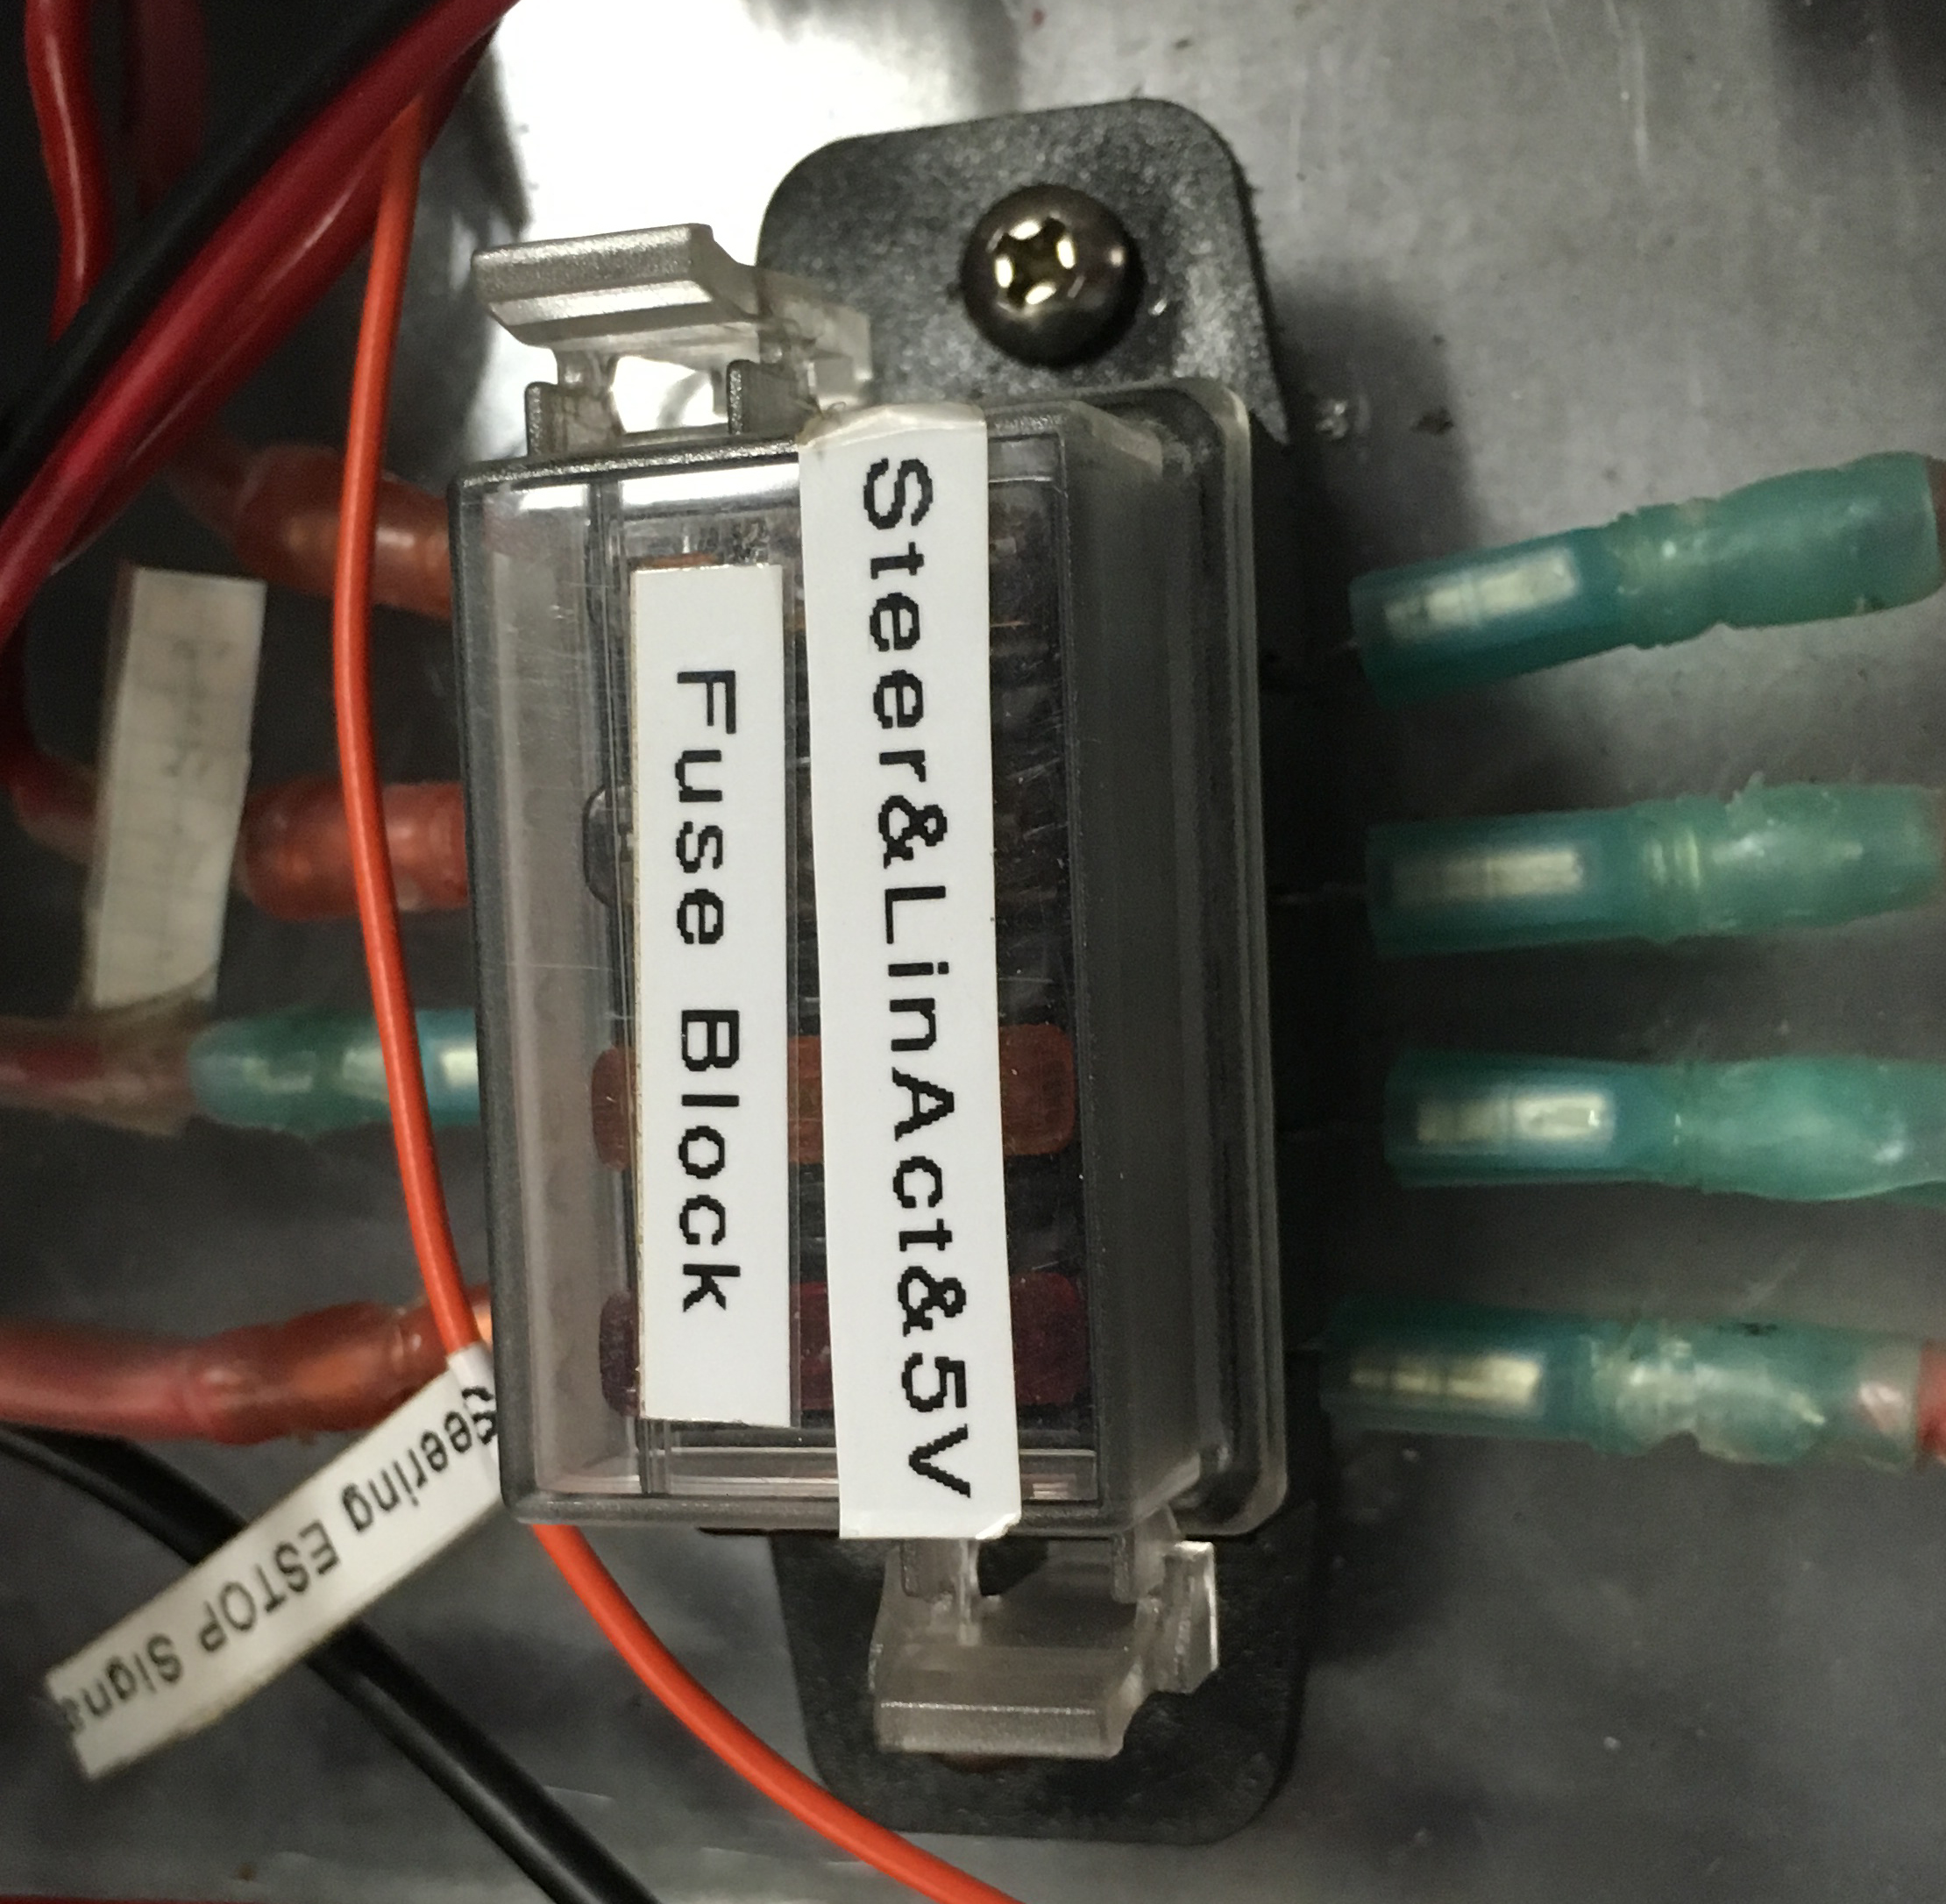
\includegraphics[scale=.06]{Photos/5vblock.jpg}
\caption{\label{fig:linear} Linear Fuse Block}
\end{figure}
\end{minipage}

\subsubsection{5V DC Power and Ground Terminal Strips}

There are two terminal strips that serve as busses for 5V DC power and ground.  The 5V DC power is used for:

\begin{enumerate}
\item Both commfronts that process serial signals from the LiDARs
\item To steering encoder
\item To cabin 5 volts
\item Signal to a 5V sensing probe
\end{enumerate}

\noindent The ground terminal strip is used for:

\begin{enumerate}
\item Ground connection for the E-Stop magnet coil
\item Ground to the 5V sensing probe
\item Ground to the E-Stop relay
\end{enumerate}
\newpage
%
\section{Overview of the Software Architecture}
The software that runs the Gator includes a stack running on Robot Operating System (ROS) on the Intel Nuc computer in Linux and a second stack running in LabVIEW on the windows 7 %rack computer. The LabVIEW code is designed to be minimally intrusive to any intelligent operation. It's sole purpose is to keep the vehicle safe and prevent the vehicle from sustaining %damage. The ROS code, on the otherhand, is designed to have most of the intelligence required for performing missions. This segregation of responsibility therefore facilitates different %teams with different mission requirements, allowing any team to run their code on the vehicle with minimal additional set up time. As long as the ROS-LabVIEW interface is obeyed, the %software architecture will support swapping out the ROS-based code at any time and the vehicle should still run.\\ \\
%
\noindent The software on the vehicle is broken up into three main parts: Forebrain, Midbrain and Hindbrain. Each part has a different function and operating speed. The hindbrain has %the fastest operating speed and is used for low-level control of the control surfaces on the vehicle such as the gas and brake pedals. As such, the hindbrain is implemented on a National %Instruments NI FPGA. The midbrain has two parts: one handling LabVIEW internal processing and another handling passing of sensor and vehicle information from LabVIEW to ROS. %Finally, the forebrain is entirely ROS-based and handles all the high-level processing tasks such as path planning and intelligent obstacle avoidance. \\ \\
%
In the upcoming sections, the various components of the software stack will be discussed in full detail.

\newpage
\chapter{Software System Definitions}

As in any large-scale system with multiple subsystems, the must be common system-level definitions that are obeyed by all subsystems. In the robot's software, too, there are common definitions obeyed by all layers of code in LabVIEW and in ROS. As such, this chapter will detail the common software system definitions.

\section{The Vehicle Co-Ordinate System}

The vehicle co-ordinate system is defined using the standard used on most ground vehicles: with the positive x direction straight ahead. In order to maintain a right-handed co-ordinate system, the three axes of the vehicle co-ordinate system are therefore defined as:

\begin{enumerate}
\item The positive X axis is pointed to the front of the vehicle
\item The positive Y axis is pointed to the left of the vehicle
\item The positive Z axis is pointed upward
\end{enumerate}

\begin{figure}[h!]
\centering
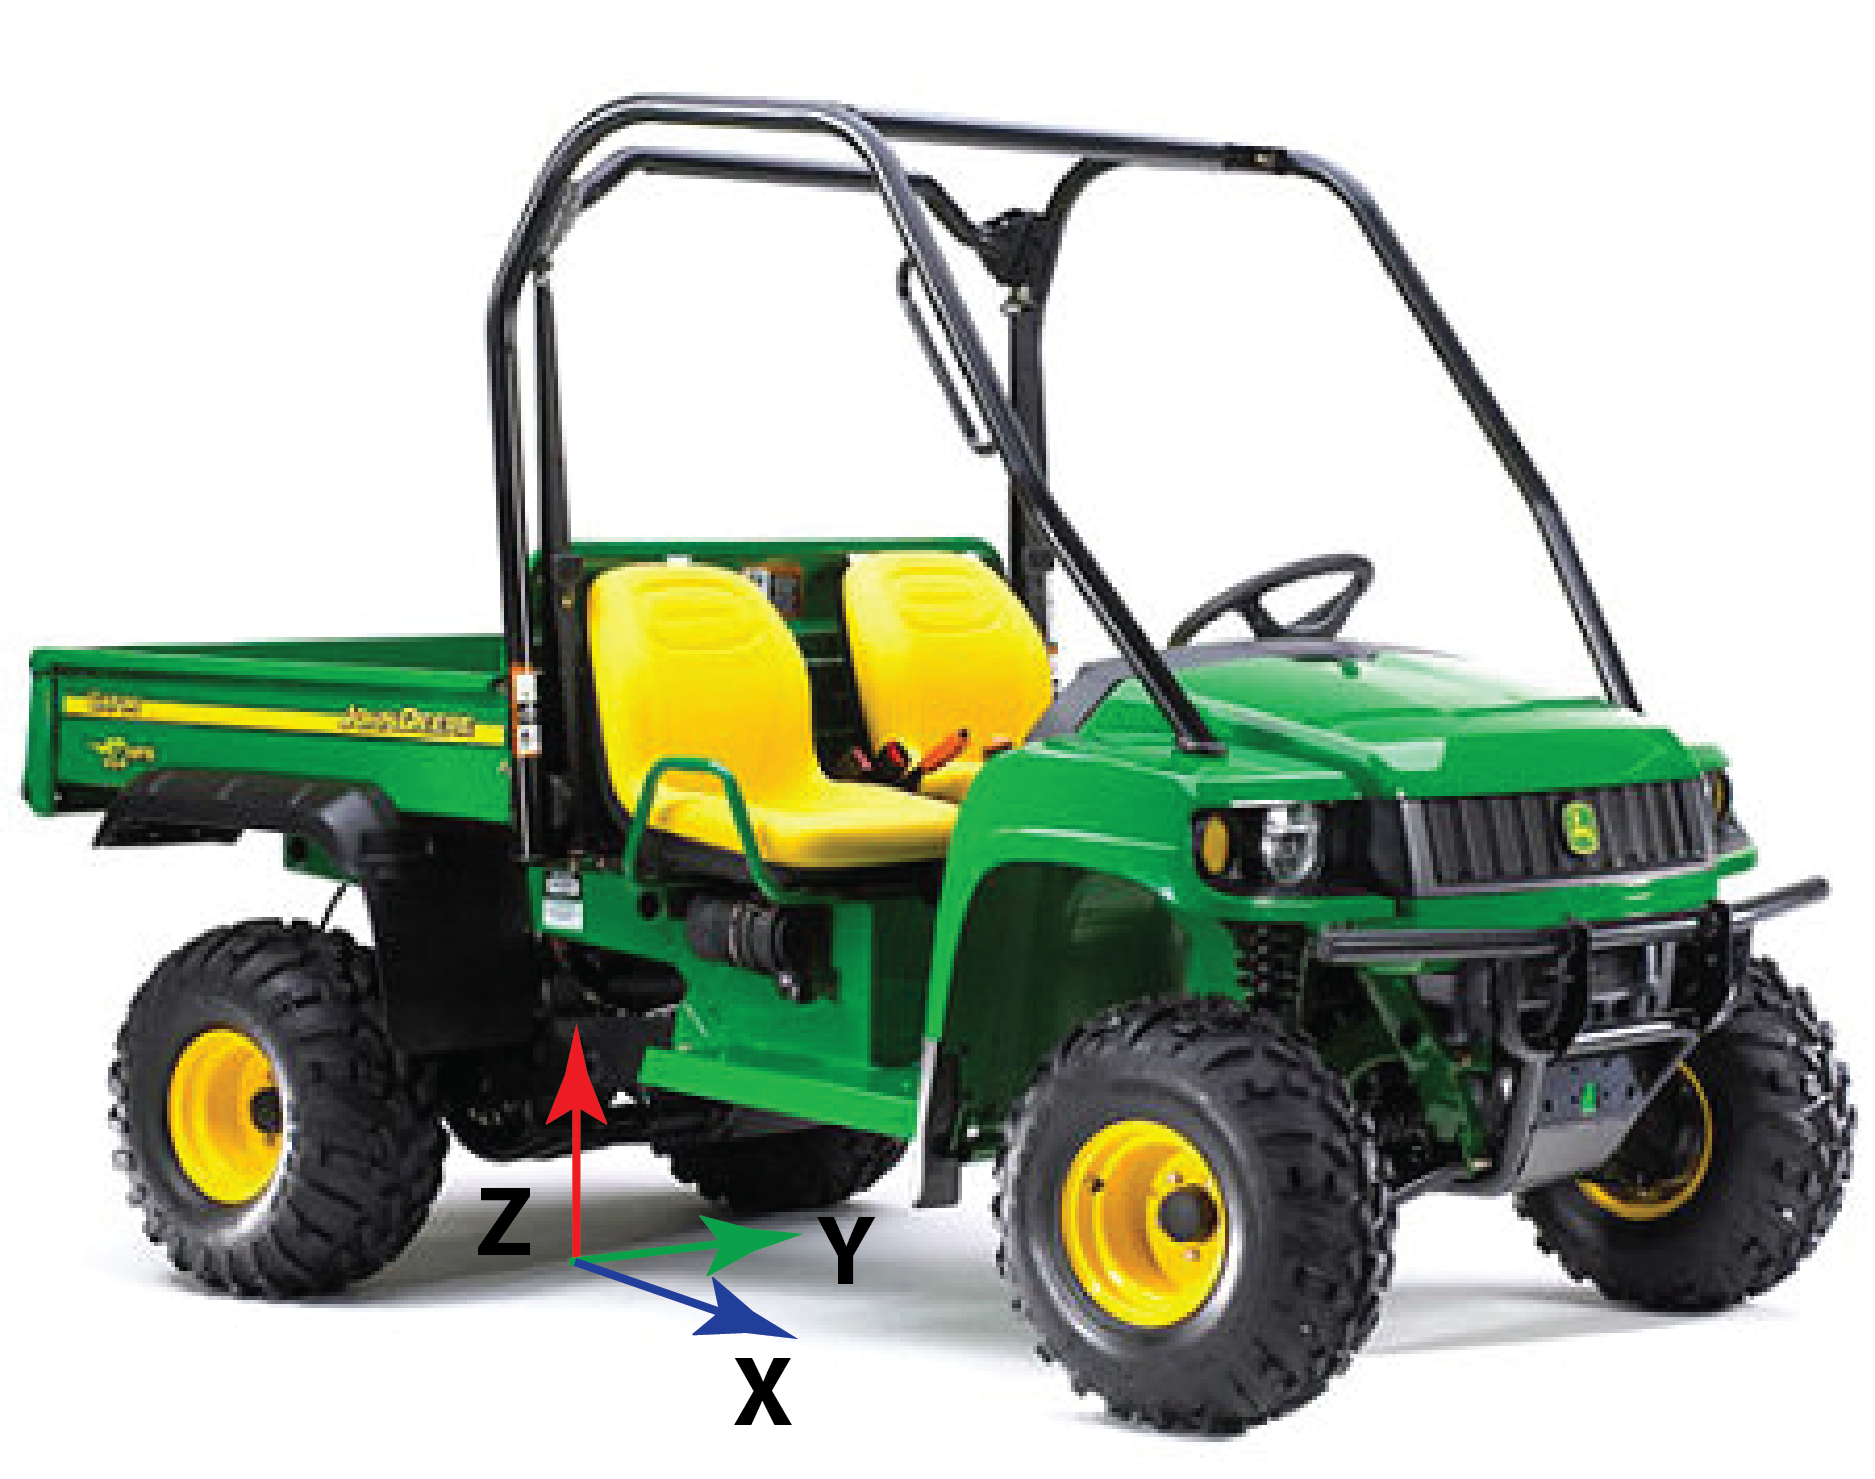
\includegraphics[scale=.7]{Photos/veh_coord.png}
\caption{Vehicle Co-ordinate System Definition}
\label{fig:veh_coord}
\end{figure} 


\newpage

\noindent The respective rotations in the vehicle co-ordinate system are therefore defined as:

\begin{enumerate}
\item Positive rotation about the X axis (Positive Roll) is roll toward the driver's right side of the vehicle
\item Positive rotation about the Y axis (Positive Pitch) is pitch downward toward the ground
\item Positive rotation about the Z axis (Positive Yaw) is yaw toward the driver's left side (counter clockwise yaw) of the vehicle
\end{enumerate}

\newpage

\section{LIDAR Co-Ordinate Definition}
By default, the Sick LMS290 LIDARs are programmed to transmit distance measurements in millimeters (mm) and angles in degrees with 0 degrees on the right and 180 degrees on the left as shown in the image below:

\begin{figure}[h!]
\centering
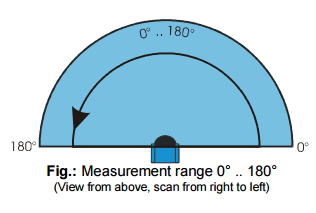
\includegraphics[scale=.9]{Photos/LIDAR_AngleDef.png}
\caption[Sick LMS290 Angle Definition]{Sick LMS290 Angle Definition \protect \footnotemark}
\label{fig:sick_angledef}
\end{figure} 
\footnotetext{ Information obtained from Quick Manual for LMS Communication Setup}
\newpage
\chapter{The Robot Software System (LabVIEW)}

In this chapter, the LabVIEW portion of the software will be discussed. Do note that there will be some features of the software such as timed while loops that will seem strange at first glance and the reason for the use of those features will not be written in this chapter. It is likely that such features are used as part of good LabVIEW FPGA programming practice and such practices will be documented in an Appendix at the end of this report. So, do remember to look at that section to fully understand the use of features such as timed while loops.

\section{The FPGA Hindbrain}
As discussed in the software overview chapter, the Hindbrain of the vehicle is implemented on a LabVIEW FPGA in order to ensure that control loops and essential data processing is done at the fastest possible speeds to reduce system latency even when the vehicle travels at higher speeds. \\ \\
%
The front panel and block diagram of the top-level hindbrain VI is shown below:

\begin{figure}[h!]
\centering
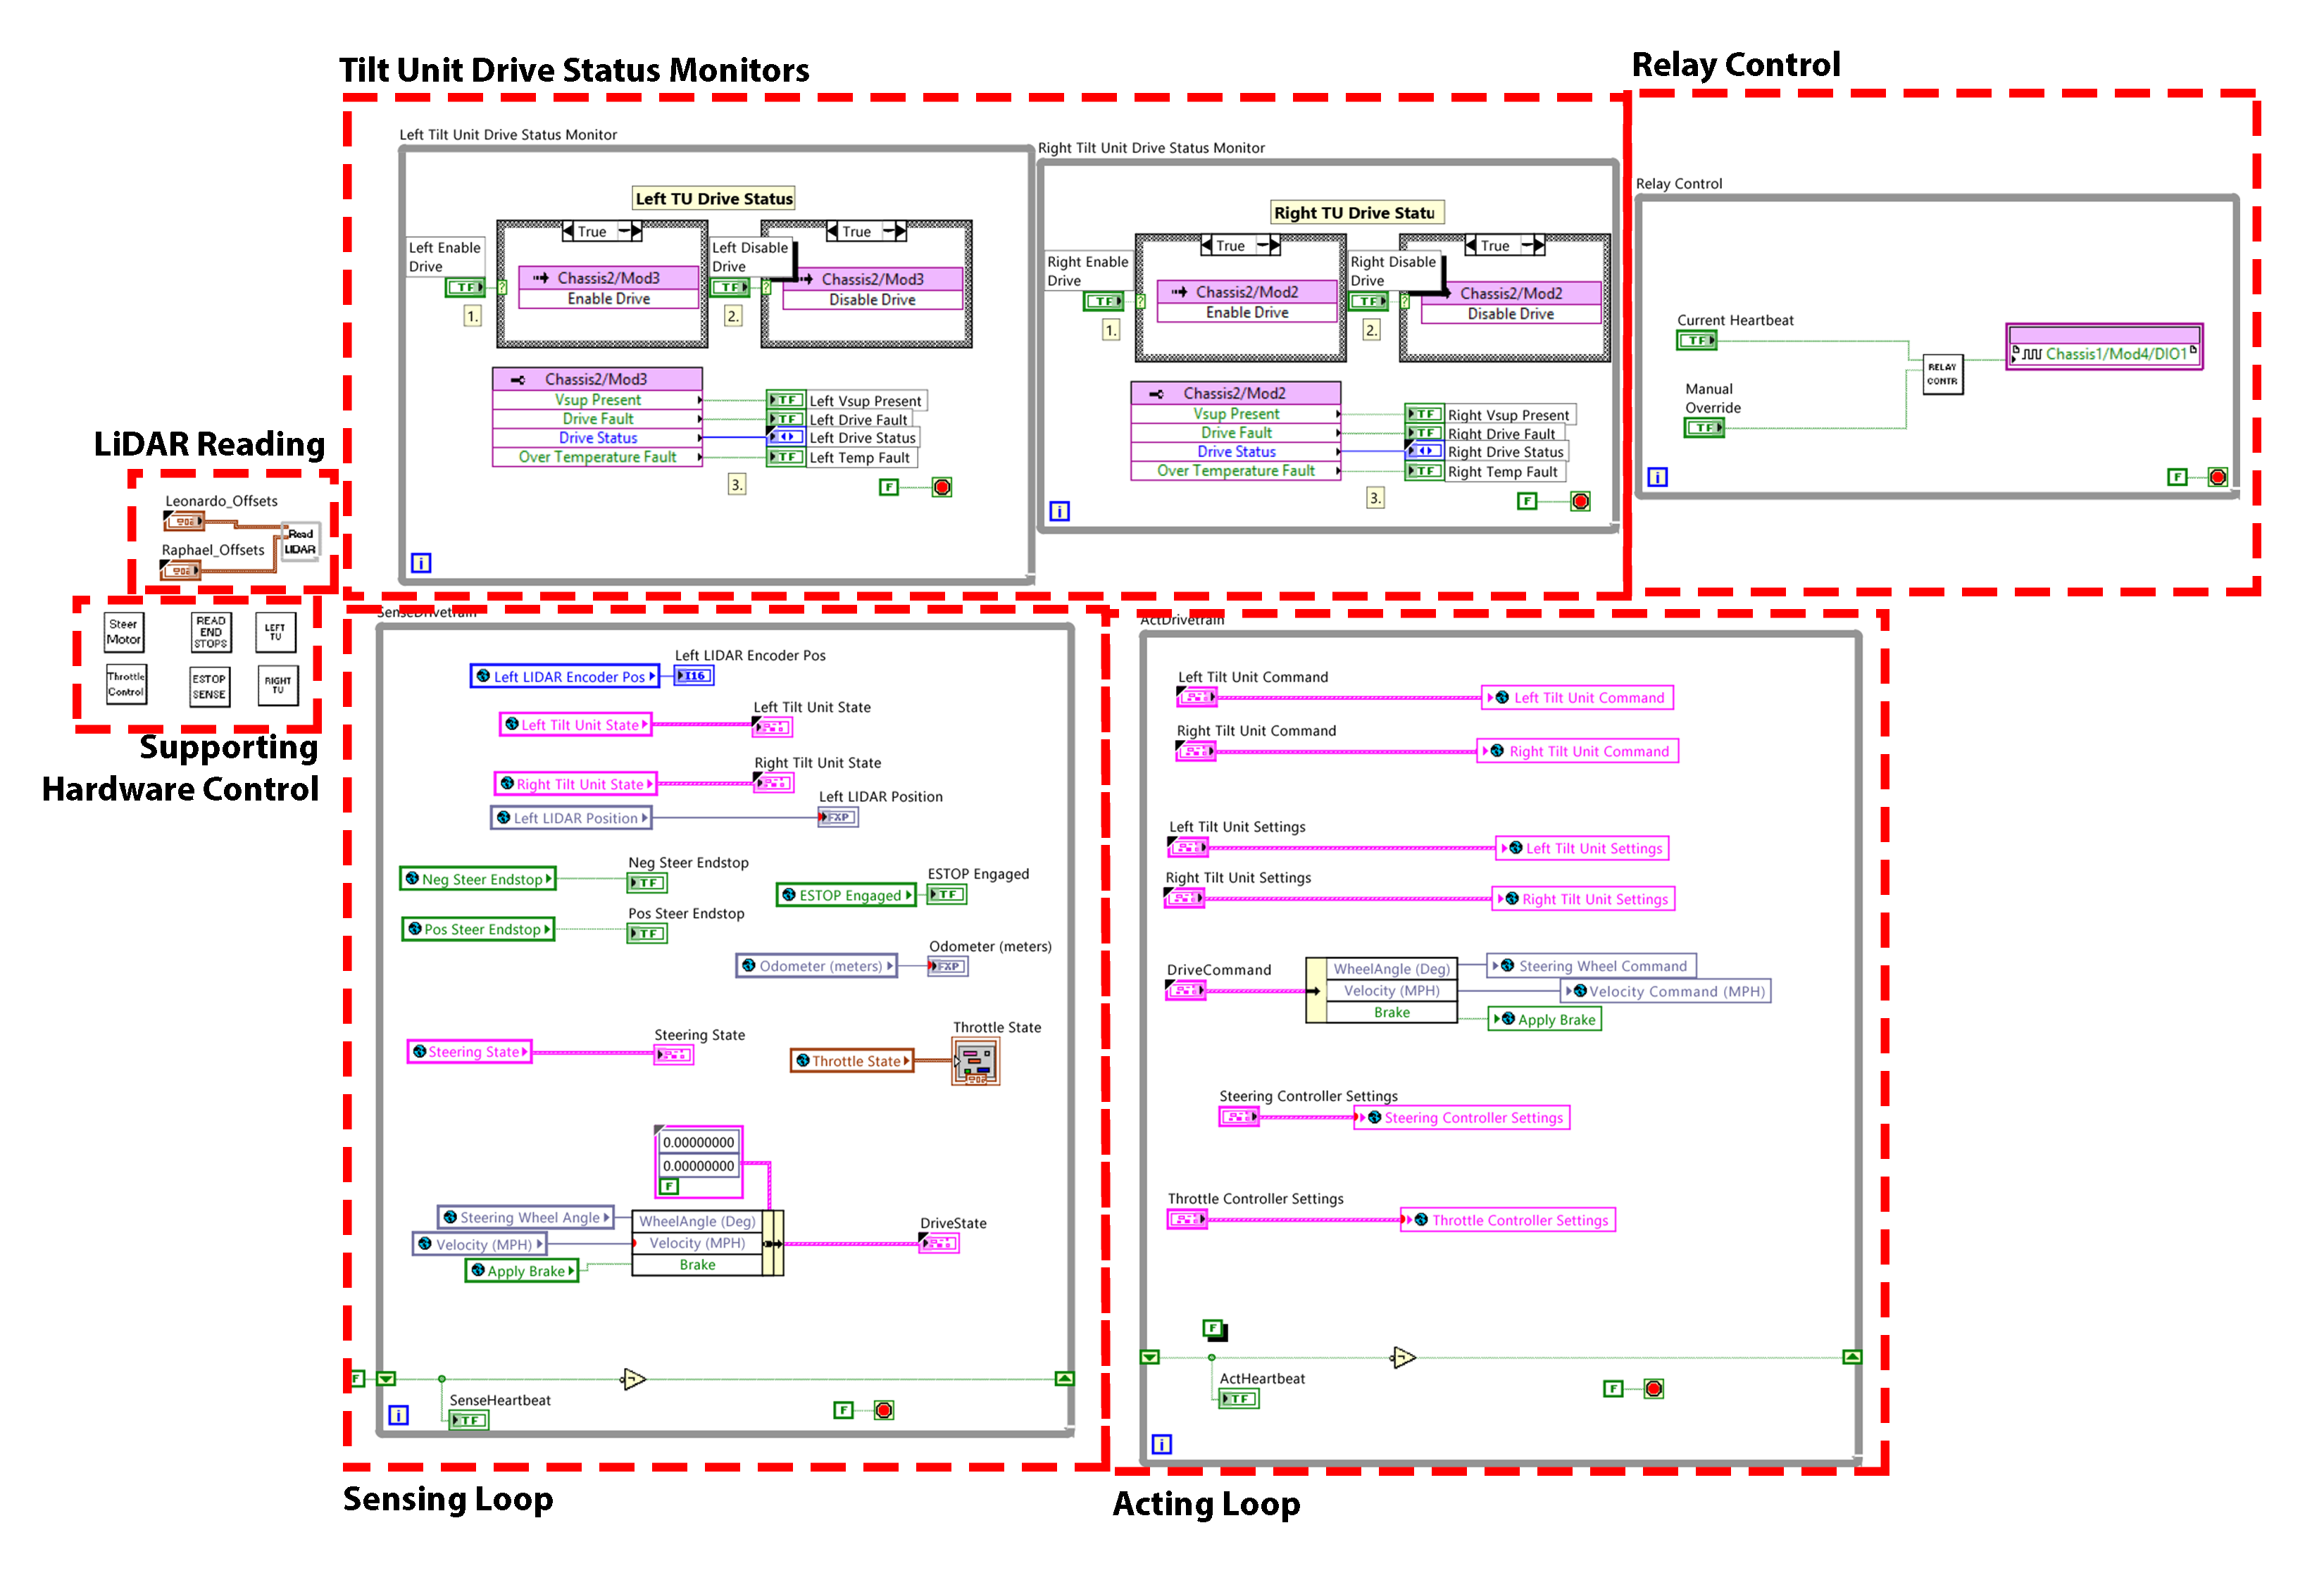
\includegraphics[scale=0.55]{Photos/hindbrainblock_annotated.png}
\caption{Hindbrain top-level VI block diagram with subchapters annotated}
\label{fig:hindbrainblock}
\end{figure} 

\newpage

\noindent As can be seen in Figure \ref{fig:hindbrainblock}, the main subchapters of the FPGA hindbrain are:

\begin{enumerate}
\item Sensing Loop
\item Acting Loop
\item Tilt Unit Drive Status Monitors
\item LiDAR Reading
\item Supporting Hardware Control
\item Relay Control
\end{enumerate}

\subsection{Sensing Loop}

The sensing loop of the FPGA hindbrain essentially passes status information and data from other parts of the FPGA hindbrain code up to the front panel so that the real-time code can access these variables. The block diagram for the sensing loop shown in Figure \ref{fig:hindbrainblock} is shown zoomed in below: 

\begin{figure}[h!]
\centering
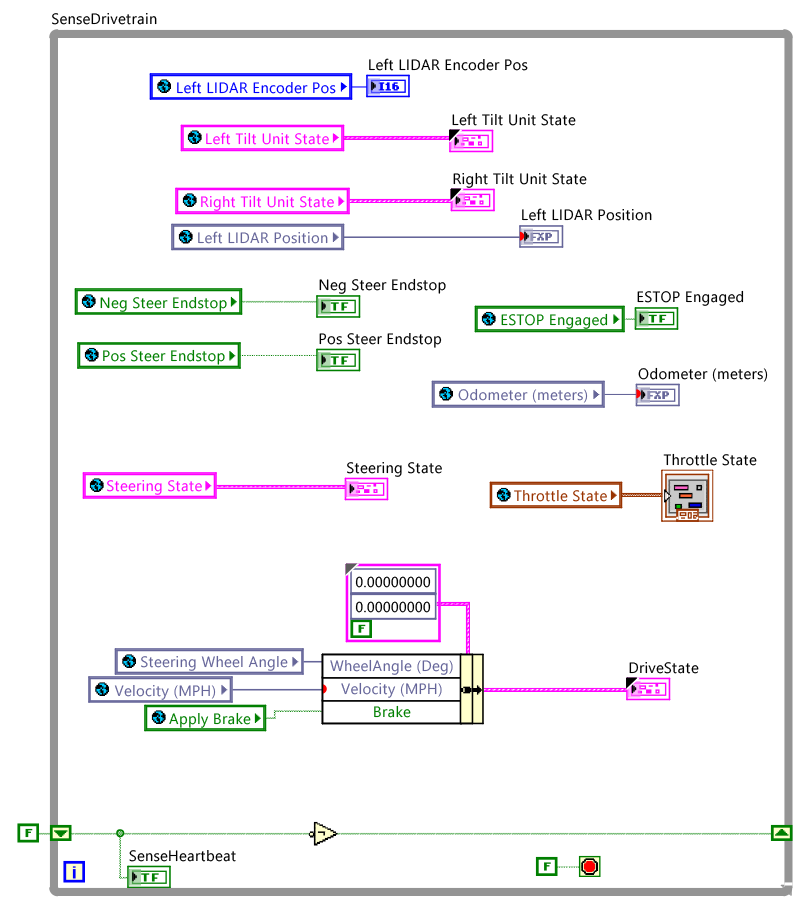
\includegraphics[scale=1.5]{Photos/sensingloop.png}
\caption{Sensing loop in the hindbrain VI}
\label{fig:sensingloop}
\end{figure} 

\noindent As shown in Figure \ref{fig:sensingloop}, the sensing loop is responsible for exposing front panel elements for the following pieces of data to the real-time code:

\begin{enumerate}
\item Left LiDAR Encoder Position: A debugging indicator that shows the encoder position of the left LiDAR in units of encoder ticks
\item Left Tilt Unit State: A cluster containing an indicator for whether the index had been found, whether the tilt unit has been told to be in initialize mode, whether there is a position error in the tilt unit and the encoder position.
\item Right Tilt Unit State: The same cluster as the left tilt unit state cluster used for the right tilt unit
\item Left LiDAR Position: Another debug indicator that shows the position of the left tilt unit in degrees after the encoder ticks have been converted to degrees
\item Negative Steer Endstop: A boolean that represents whether the negative steer angle endstop has been triggered
\item Positive Steer Endstop: A boolean that represents whether the positive steer angle endstop has been triggered
\item Estop Engaged: A boolean that represents whether either of the physical estop buttons have been triggered
\item Odometer (meters): The distance travelled by the vehicle since the code started running
\item Throttle state: A cluster containing indicators for the gas and brake pedal voltage being sent to the linear actuators for the gas and brake respectively
\item DriveState: A cluster indicating the driving state of the vehicle including the steering wheel angle in degrees, the velocity in miles per  hour and the boolean that represents whether the vehicle should apply the brakes
\item SenseHeartBeat: An indicator that simply provides a blinking light that confirms the while loop is running 
\end{enumerate}

\subsection{Acting Loop}

The acting loop of the FPGA hindbrain essentially performs the opposite function of the sensing loop: to provide indicators for the real-time code to pass commands or instructions down to the FPGA code. The block diagram for the acting loop shown in Figure \ref{fig:hindbrainblock} is shown zoomed in below:

\newpage

\begin{figure}[h!]
\centering
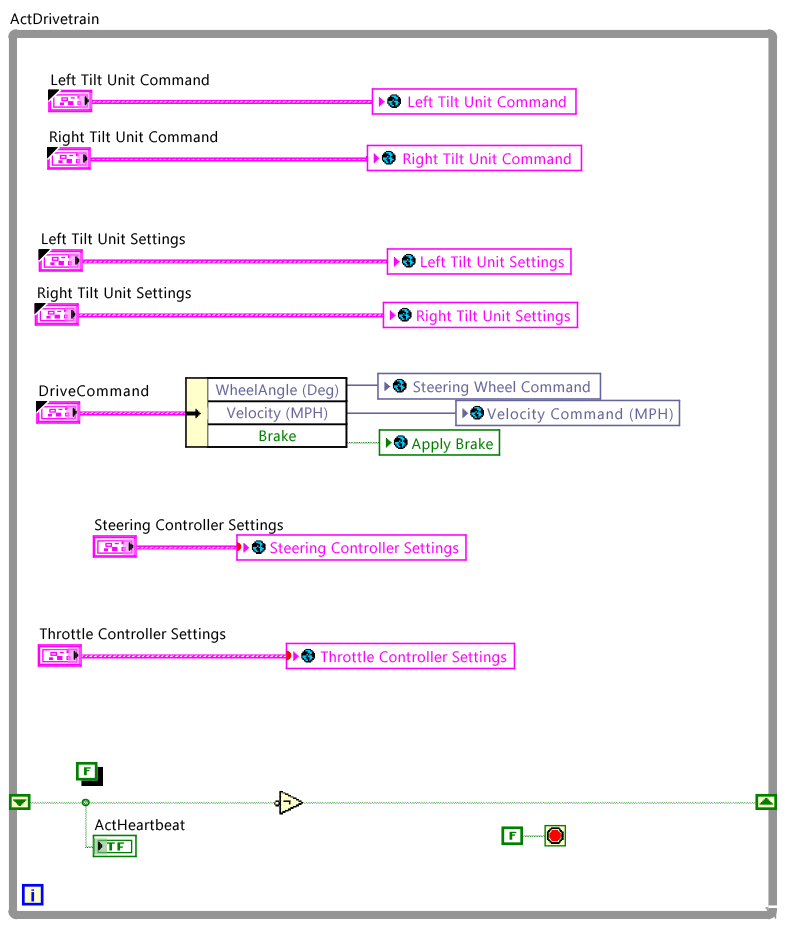
\includegraphics[scale=1.5]{Photos/actloop.png}
\caption{Acting loop in the hindbrain VI}
\label{fig:actloop}
\end{figure}

\noindent As shown in Figure \ref{fig:actloop}, the acting loop is responsible for providing front panel elements for the real-time code to send the following commands to the FPGA code:

\begin{enumerate}
\item Left Tilt Unit Command: A cluster that contains indicators for whether the tilt unit should be in initialize mode, the position setpoint of the tilt unit in degrees, the current output when the tilt unit is in initialize mode and a reset position boolean that indicates whether the position of the tilt units should be reset to zero.
\item Right Tilt Unit Command: The same cluster as Left Tilt Unit Command, but for the right tilt unit
\item Left Tilt Unit Settings: A cluster that contains the controller settings for the left tilt unit including the position proportional, integral and derivative (PID) gains, Current PI gains and the current limit
\item Right Tilt Unit Settings: The same settings cluster as the Left Tilt Unit Settings for the right tilt unit
\item Drive Command: A cluster containing the desired wheel angle in degrees, the desired velocity in miles per hour and a boolean to command the vehicle to apply the brakes
\item Steering Controller Settings: A cluster containing the controller settings for the steering control including the PID gains, upper and lower voltage limits, upper and lower encoder limits, PID to motor conversion constant, motor deadband high and low threshold, a reset position boolean for resetting the steer motor position and two other booleans to tell the vehicle whether to allow positive and negative steering voltages or not.
\item Throttle Controller Settings: Cluster containg the throttle controller settings for the gas and brake controllers including the PID gains for the gas pedal controller, voltage offset that indicates the neutral position voltage, position reset and PID reset boolean, maximum and minimum brake voltage, maximum and minimum gas pedal voltage and the speed of the throttle control loop. 
\end{enumerate}

\subsection{Tilt Unit Drive Status Monitors}
The tilt unit drive status monitors essentially provide inputs and outputs that allow the real-time code to command the NI9505 motor control modules and receive information on the status of the modules. The block diagram for the tilt unit drive status monitors shown in Figure \ref{fig:hindbrainblock} is shown zoomed in below:

\newpage

\begin{figure}[h!]
\centering
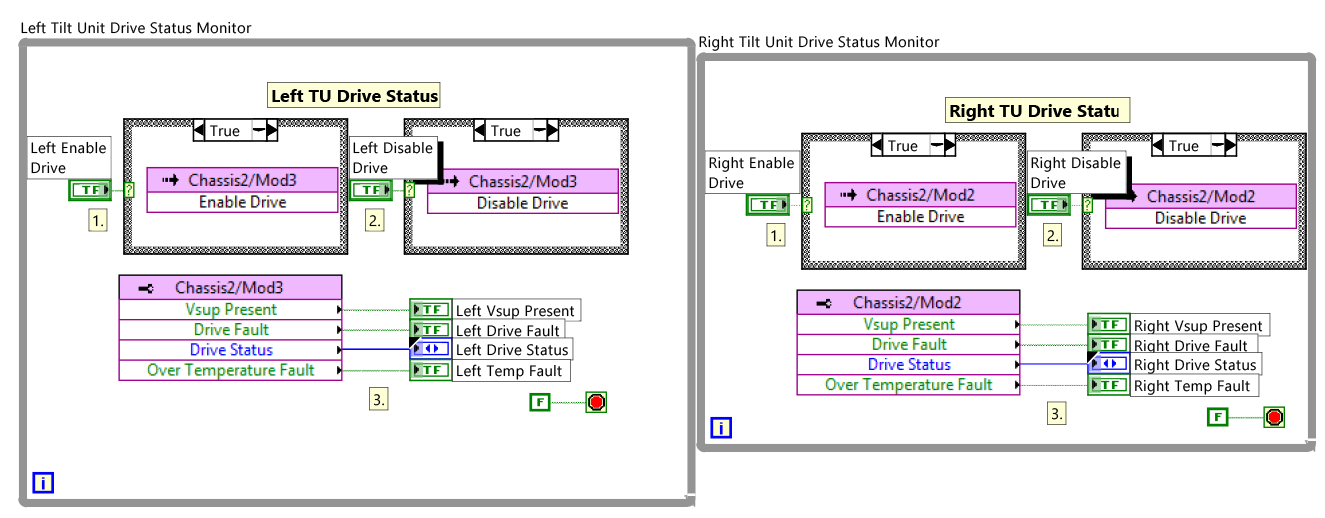
\includegraphics[scale=1.2]{Photos/tudrivestat.png}
\caption{Tilt unit drive status monitors in the hindbrain VI}
\label{fig:tudrivestat}
\end{figure}

\noindent As can be seen in Figure \ref{fig:tudrivestat}, the left and right drive status loops are basically identical to each other except for the module assignments since the left drive status monitor addresses the NI9505 module for the left tilt unit and the right drive status monitor addresses the other NI9505 module. \\ \\
%
Each drive status monitor loop contains a method for enabling the drive, disabling the drive and monitoring the presence of a power supply (vsup Present), whether the drive has a drive fault (Drive Fault), determining whether the drive is enabled or disabled (Drive Status) and whether the drive is overheating (Over Temperature Fault). By default, the NI9505 modules will be disabled when the vehicle is first powered up and so the drive will need to be enabled in software during initialization. 

\subsection{LiDAR Reading}

Although LiDAR reading shows up on the front panel of the Hindbrain top-level VI as one subVI, the process of reading data from the two Sick LMS291 LiDARs really involves several different subVIs to perform the various tasks. In summary, the process of reading data from the LiDARs involves:

\begin{enumerate}
\item Initializing the LiDARs
\item Read the raw data from the LiDARs
\item Parse and transform the LiDAR data into the vehicle's coordinate system
\end{enumerate}

\noindent On the hindbrain top-level VI, the block diagram for reading the LiDARs shown in Figure \ref{fig:hindbrainblock} is shown zoomed in below:

\begin{figure}[h!]
\centering
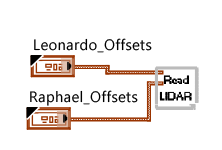
\includegraphics[scale=2]{Photos/lidarread.png}
\caption{LiDAR Reading SubVI in the hindbrain VI}
\label{fig:lidarread}
\end{figure}

\noindent As can be seen in Figure \ref{fig:lidarread}, the lidar reading VI takes the offsets for the left (Leonardo) and right (Raphael) LiDARs that provide the translations and rotations that are needed to transform the LiDAR data in the last step of the LiDAR reading process.\\ \\
%
The block diagram of the LiDAR reading VI is shown below:

\begin{figure}[h!]
\centering
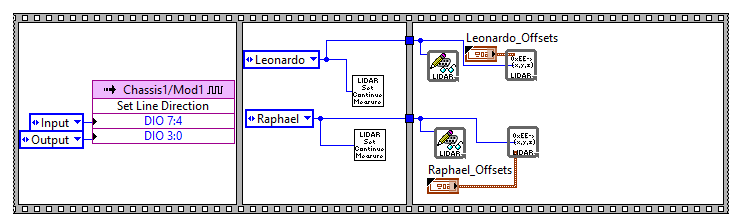
\includegraphics[scale=0.75]{Photos/readlidarblock.png}
\caption{Block diagram for the Lidar Reading VI}
\label{fig:readlidarblock}
\end{figure}

\noindent As can be seen in Figure \ref{fig:readlidarblock}, the LiDAR reading VI consists of a flat sequence with three parts:

\begin{enumerate}
\item The first part is an FPGA I/O method node that sets the the input and output lines
\item The second part contains a VI for the left and right LiDAR that sends the commands specified in the LiDAR communication protocol to tell the LiDAR to send data continuously at 25Hz
\item The third part contains two subVIs: a serial read/write VI that writes the required commands to the LiDAR and receives the LiDAR data back and a transformer VI that transforms the LiDAR data coordinate system from the LiDAR's local coordinate system to the vehicle's coordinate system.
\end{enumerate}

\subsection{LiDAR Serial Read/Write}

The block diagram for the LiDAR serial read/write VI is shown below:

\begin{figure}[h!]
\centering
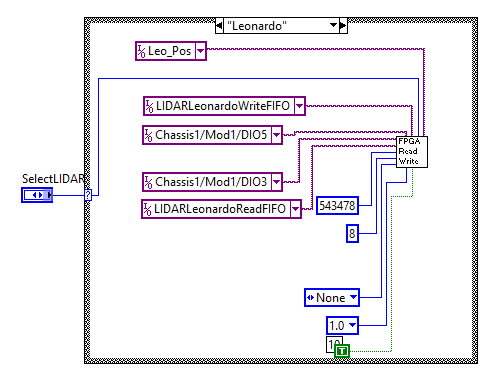
\includegraphics[scale=0.75]{Photos/readlidar_block.png}
\caption{Block diagram for the Lidar Reading VI}
\label{fig:readlidar_block}
\end{figure}

\noindent As can be seen in Figure \ref{fig:readlidar_block}, the VI is essentially a wrapper for the actual FPGA read/write functions that allows the code to reuse the same read/write functions while being able to assign the inputs and outputs to the appropriate LiDARs (either left or right). The VI takes either the left (Leonardo) or right (Raphael) LiDAR name as input and assigns the following variables to the write function:

\begin{enumerate}
\item LIDARLeonardoWriteFIFO: A First In First Out (FIFO) queue that queues the LiDAR commands to be sent to the LiDAR 
\item Chassis1/Mod1/DIO3: The DIO chanel from which LiDAR data is transmitted
\item 543478: The baud rate for LiDAR communication
\item 8: Data bits for the LiDAR
\item None: Parity for the LiDAR
\item  1.0: Stop bits
\item True boolean: Reverse Polarity command for the LiDAR
\end{enumerate}

\noindent The read function is then assigned the following variables:

\begin{enumerate}
\item LeoPos: A FIFO queue that queues the lidar position data to be read by the transformer VIs
\item Chassis1/Mod1/DIO5: The DIO channel from which LiDAR data is received
\item LIDARLeonardoReadFIFO: THe FIFO queue that queues the received LiDAR data
\item 543478: The baud rate for LiDAR communication
\item 8: Data bits for the LiDAR
\item None: Parity for the LiDAR
\item  1.0: Stop bits
\item True boolean: Reverse Polarity command for the LiDAR
\end{enumerate}

\noindent These variables are then passed down to the actual serial write and read functions as shown below:

\newpage

\begin{figure}[h!]
\centering
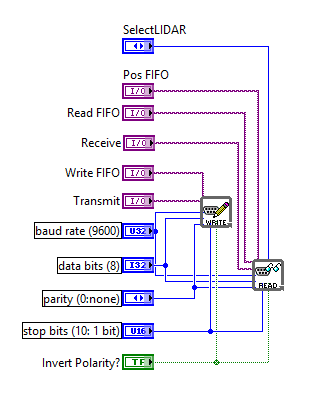
\includegraphics[scale=0.75]{Photos/readwriteblocks.png}
\caption{Block diagram for the VI providing the actual read/write functions}
\label{fig:readwriteblocks}
\end{figure}

\noindent The serial write VI is a stock serial write VI provided by LabVIEW for the LiDARs that has been modified to include a while loop around the entire serial write sequence for the LiDARs. Therefore, for brevity in this report, the write VI will not be explained in detail. However, for convenience, the documentation for the serial write VI is shown in the figure below:

\begin{figure}[h!]
\centering
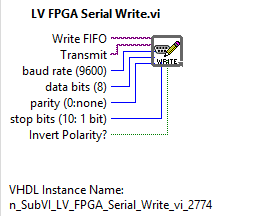
\includegraphics[scale=0.75]{Photos/writedocs.png}
\caption{Documentation for the serial write function}
\label{fig:writedocs}
\end{figure}

\newpage

\noindent The block diagram for the serial read VI, then, is shown in the diagram below:

\begin{figure}[h!]
\centering
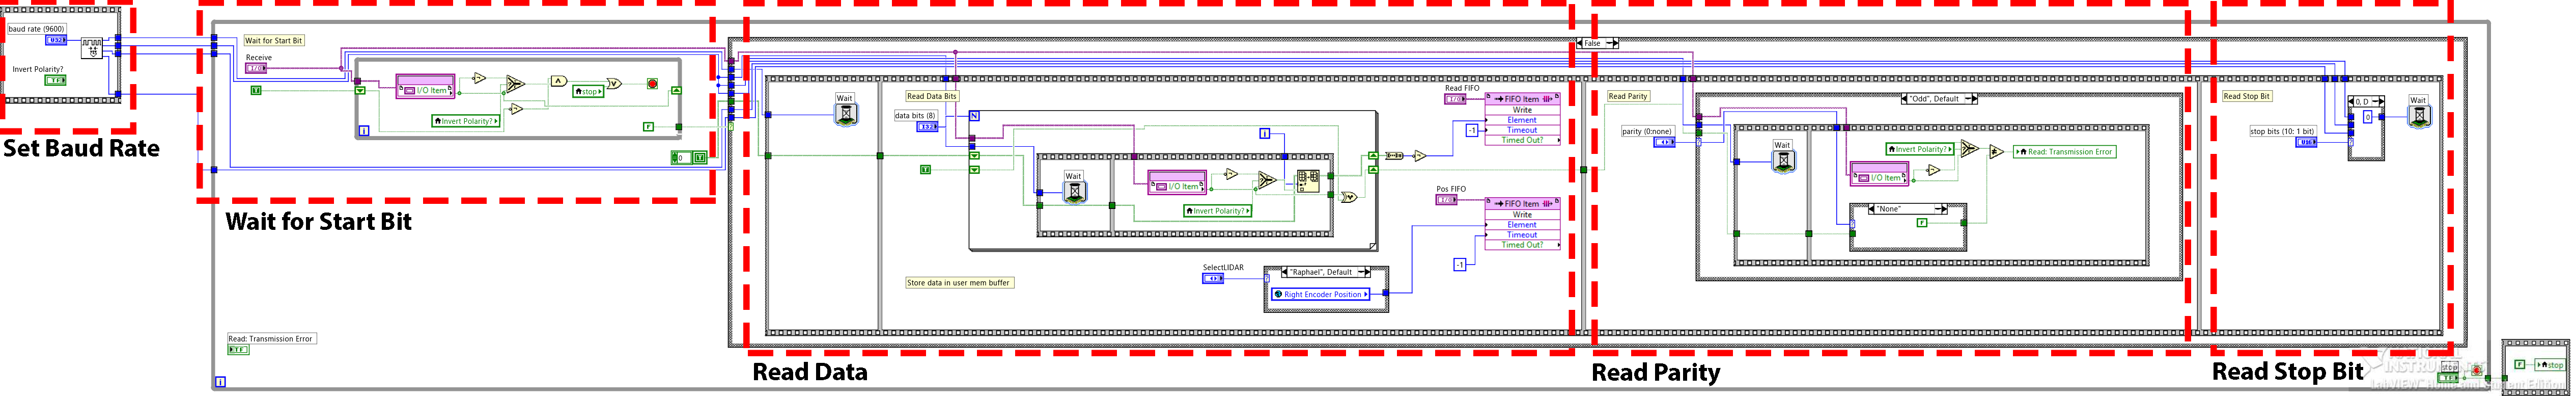
\includegraphics[scale=0.35]{Photos/serialreadblock.png}
\caption{Block diagram for the serial read function}
\label{fig:serialreadblock}
\end{figure}

\noindent As can be seen in Figure \ref{fig:serialreadblock}, after setting the baud rate, the VI executes a series of steps each time throug the while loop to receive the bits that make up the LiDAR data that is received:

\begin{enumerate}
\item Wait for the start bit of the data
\item Read data
\item Read stop bit
\end{enumerate}

\noindent For brevity, this report is not going to discuss the code that waits for the start bit or the code that reads the stop bit. When zoomed in, the read data chapter of the code is as follows:

\begin{figure}[h!]
\centering
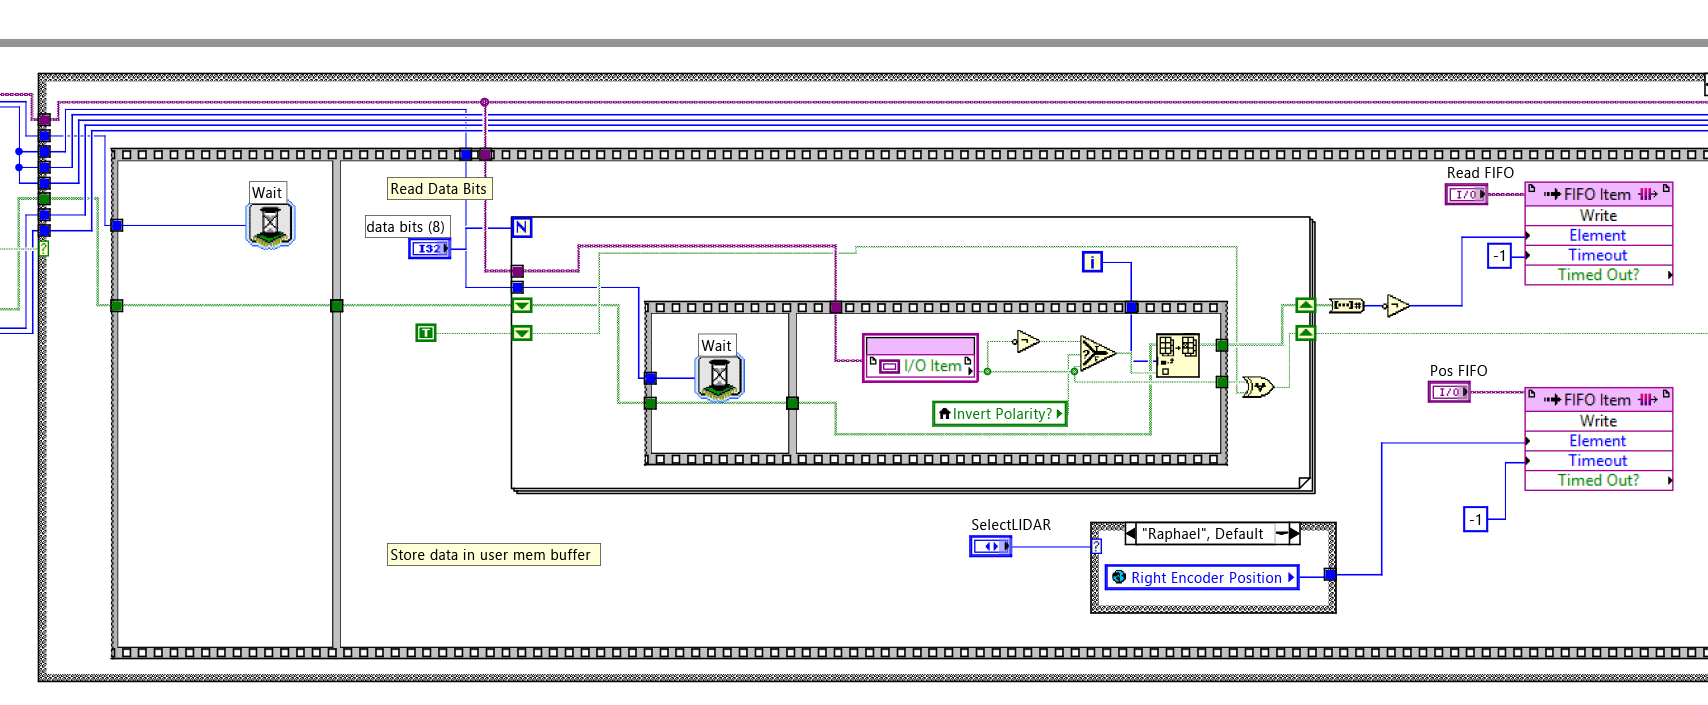
\includegraphics[scale=0.85]{Photos/readdatasection.png}
\caption{Block diagram for the chapter that reads the LiDAR data bits}
\label{fig:readdatachapter}
\end{figure}

\newpage

\noindent As can be seen in Figure \ref{fig:readdatachapter}, the data reading code essentially reads each bit as a boolean and adds it to the array. Once the for loop has been through all the bits in the mesage, it converts the data and adds it to the read FIFO queue that queues up the LiDAR reading to be read by the transforming code. At the same time, code in parallel reads either the left or right encoder position (depending on whether Raphael or Leonardo is selected) and and appends the encoder tick count to a separate position FIFO queue to be read by the transformer code.

\subsection{LiDAR Data Transform}
After the LiDAR read/write functions, the next step in processing the LiDAR data is to transform it from the local LiDAR coordinate system to the vehicle coordinate system. 

\subsubsection{LiDAR Parse Transform and Send VI}
Referring back to Figure \ref{fig:readlidarblock}, the block on the far right is the VI that parses the LiDAR data, transforms it and then sends it over a FIFO queue up to the real-time layer. The block diagram for this VI is shown below:

\begin{figure}[h!]
\centering
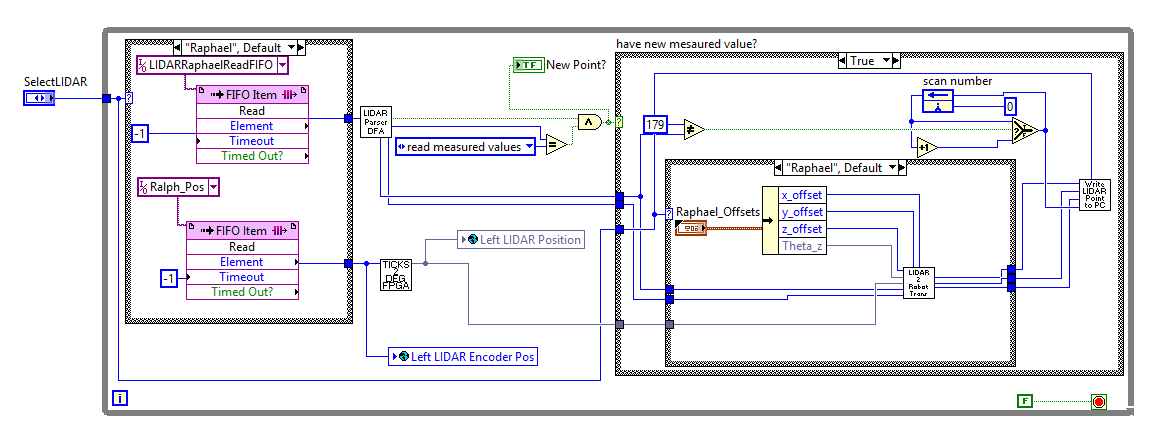
\includegraphics[scale=0.5]{Photos/lidartransformandsend.png}
\caption{Block diagram for the Parse Transform and Send VI}
\label{fig:parseandsend}
\end{figure}

\noindent As shown in Figure \ref{fig:parseandsend}, the transform and send VI runs a while loop that is constantly processing LiDAR data coming from the FIFO queues that was written to those queues by the LiDAR serial read/write VIs. Data from the upper FIFO queue (the LiDAR data read from the LiDAR) is passed through a LiDAR data parser that parses each piece of data, parses the checksum and other additional data in the LiDAR data, including the distance reading and the scan number. The scan number is sent up to the real-time layer and the distance reading is then sent to the next subfunction in the parse transform and send VI. \\ \\
%
The data from the lower FIFO queue (the position of the LiDAR in encoder ticks), then, is passed through a function that converts the encoder ticks to LiDAR position in degrees. That LiDAR position data is then passed to the next part of the transform code as the y-axis rotation (pitch).

\subsubsection{LiDAR to Robot Transform: Overview}
As shown in Figure \ref{fig:parseandsend}, the next step in the transform process is the transform itself. The data returned by the Sick LMS290 LIDARs is in the co-ordinate frame of the LIDARs by virtue of the way in which the LIDARs take readings. In order to do useful work with the LIDAR data, the LIDAR data has to be transformed to make it iwth reference to the vehicle co-ordinate system.

\subsubsection{Constant LIDAR Transform Properties}
Based on the design and placement of the LIDAR mounts, the following properties of the LIDAR transform are applied to make the transform:

\begin{enumerate}
\item For the left side LiDAR, the constant transforms are:
\begin{enumerate}
\item X translation: 2000mm
\item Y translation: 450mm
\item Z translation: 1000mm
\item Z rotation (yaw): 45 degrees
\end{enumerate}
\item For the right side LiDAR, the constant transforms are:
\begin{enumerate}
\item X translation: 2000mm
\item Y translation: -450mm
\item Z translation: 1000mm
\item Z rotation (yaw): -45 degrees
\end{enumerate}
\end{enumerate}

\noindent The observant reader will note that the Y rotation (pitch) of the LiDARs is nto a constant property and depends on the encoder tick count. This will be explained in more detail in the later sections. 

\subsubsection{The LiDAR Transform VI}

The block diagram for the LiDAR transform VI is shown below:
\begin{figure}[h!]
\centering
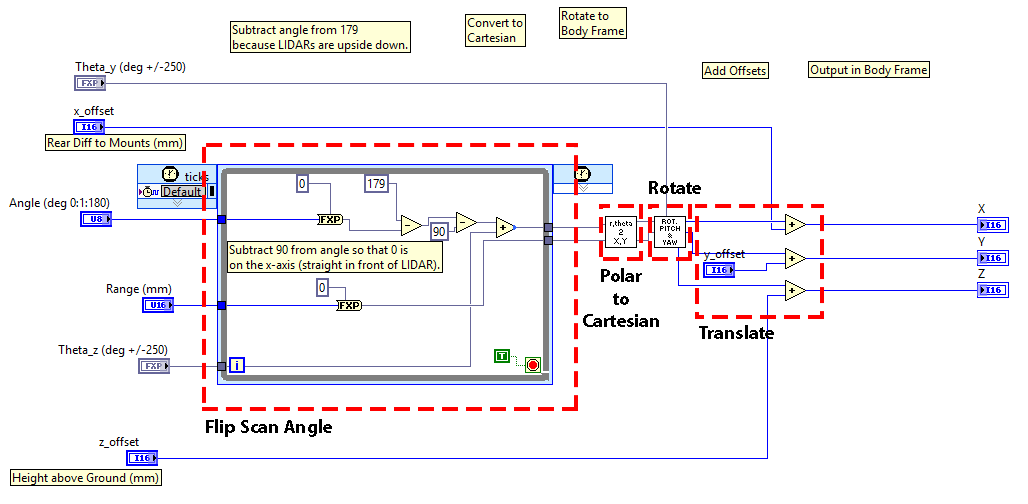
\includegraphics[scale=0.5]{Photos/transformvi.png}
\caption{Block diagram for the LiDAR transform VI}
\label{fig:transformvi}
\end{figure}

\noindent As can be seen in Figure \ref{fig:transformvi}, the transform process has four parts:

\begin{enumerate}
\item Flip the scan angle over to account for the LiDAR being mounted up-side-down and place 0 degrees in the center of the scan (i.e. such that 0 is in the center of the scan, 90 degress is on the right and -90 degrees is on the left 
\item Convert each scan from polar co-ordinates to cartesian co-ordinates
\item Rotate the coordinate frames such that the frame local to the LIDAR is in the same orientation as the vehicle co-ordinates
\item Translate the coordinate frames such that the frame local to the LIDAR is translated to line up with the vehicle co-ordinate system
\end{enumerate}

\noindent The rotations are necessary to align the local LiDAR coordinate axes with the vehicle coordinate axes. This is illustrated in the figure below:

\begin{figure}[h!]
\centering
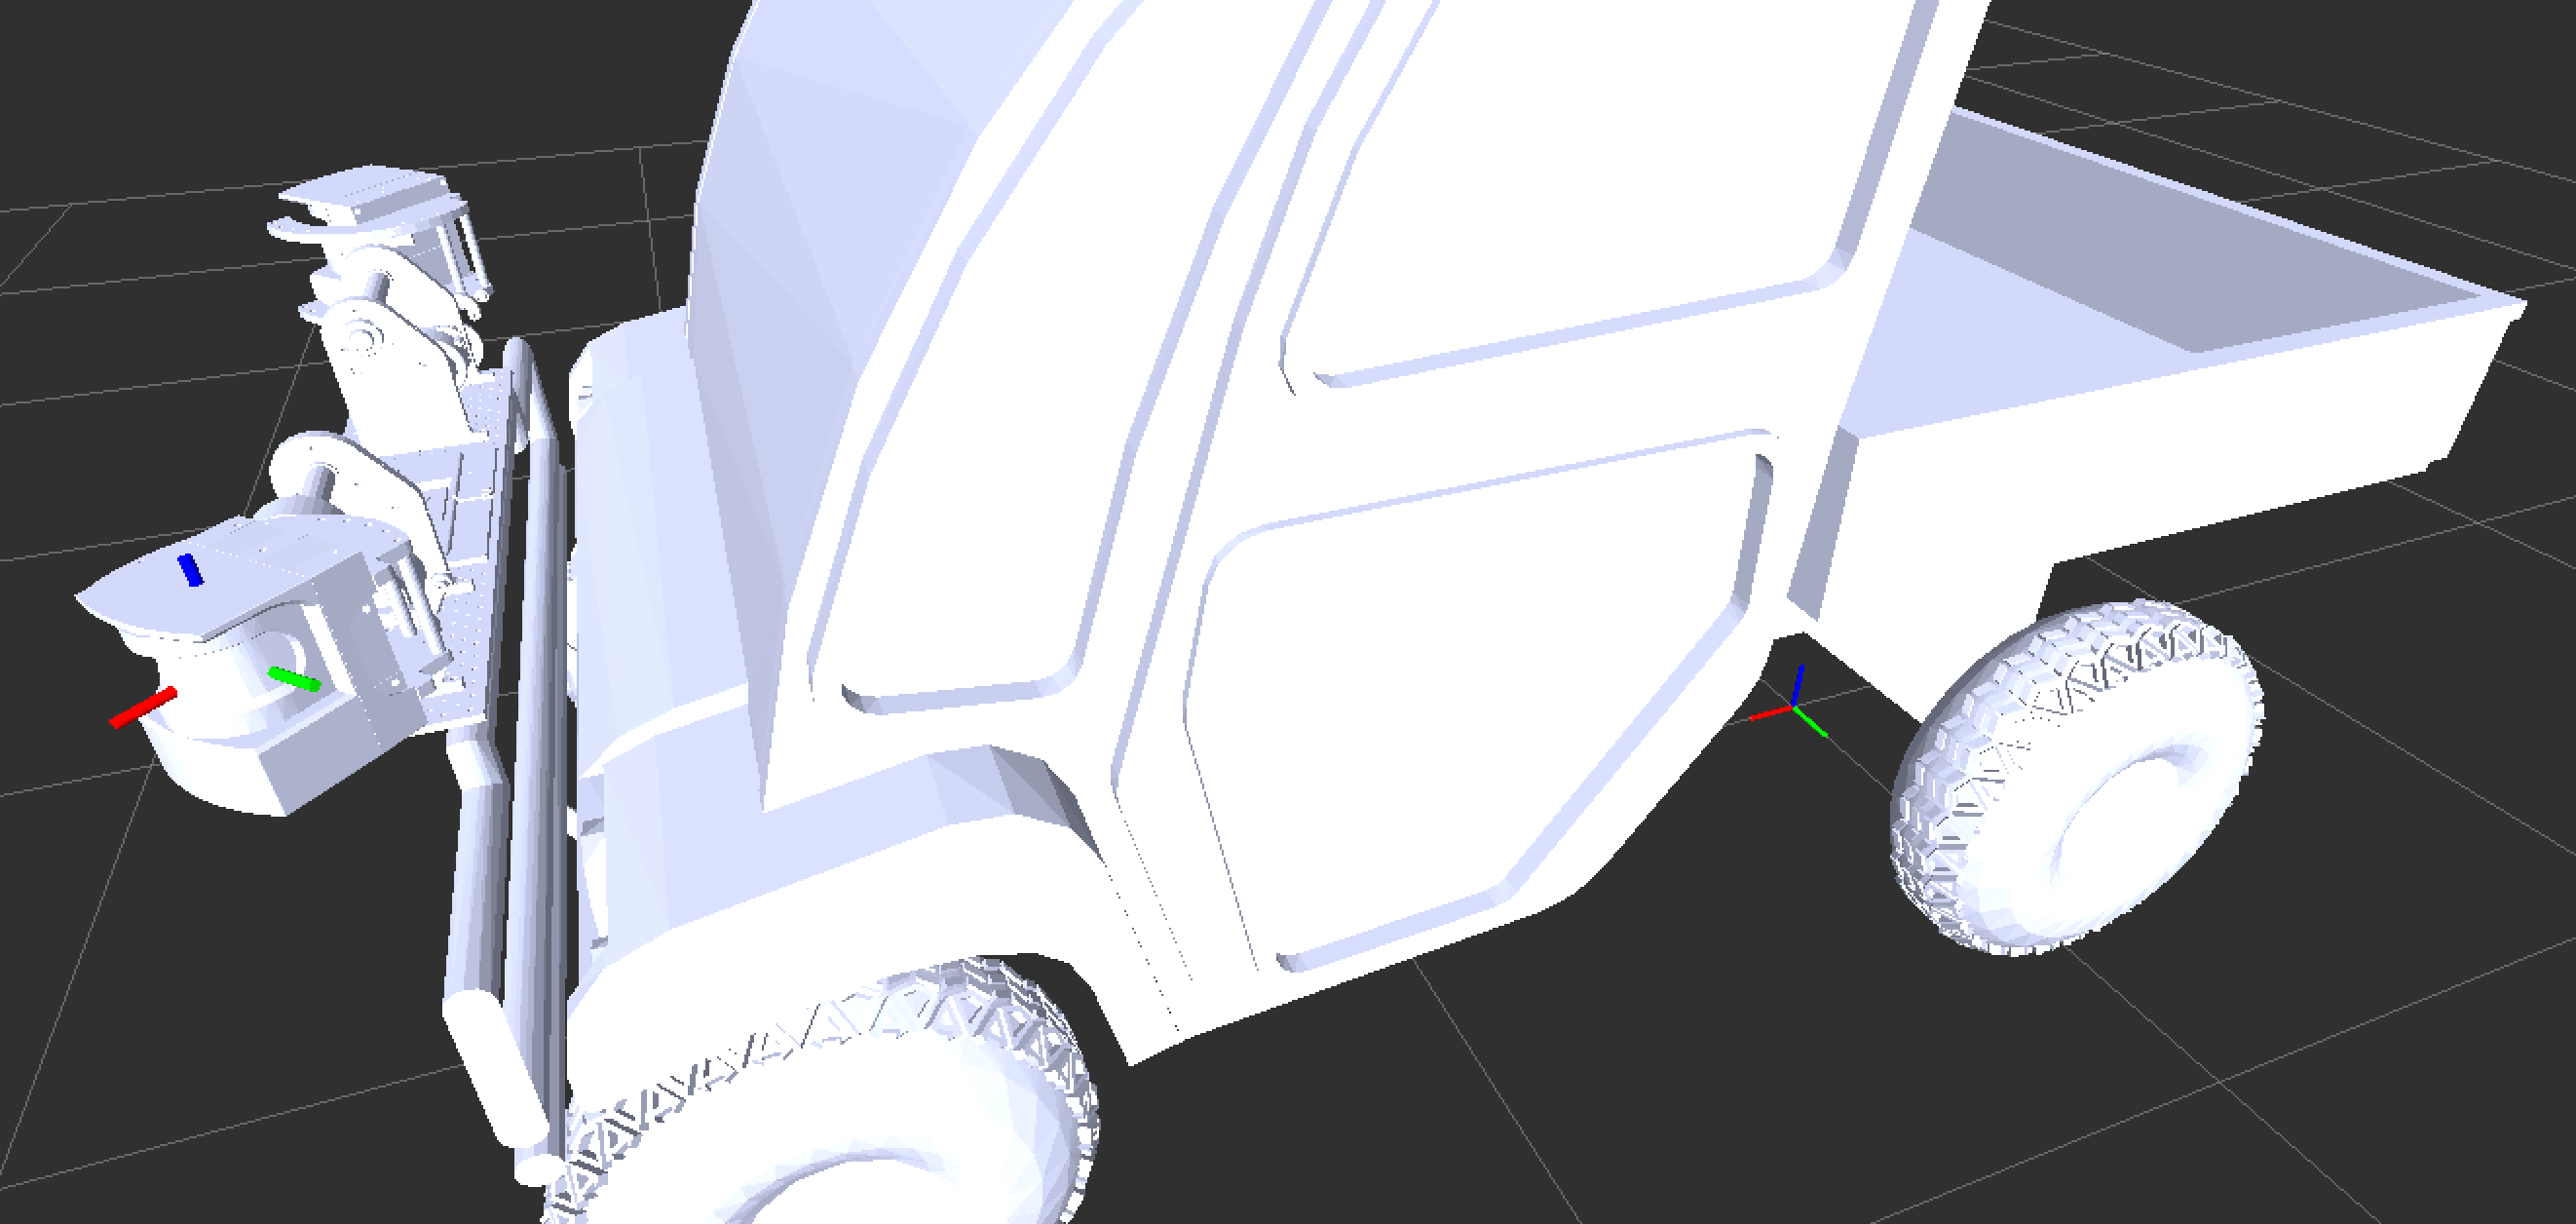
\includegraphics[scale=0.3]{Photos/lidarrobotaxes.png}
\caption{Diagram showing the LiDAR local axes (in the center of the LiDAR) and the vehicle axes (on the ground below the rear axle of the vehicle); X is red, Y is green, Z is blue}
\label{fig:lidarrobotaxes}
\end{figure}

\noindent As can be seen in Figure \ref{fig:lidarrobotaxes}, the local coordinate system of the LiDAR is rotated relative to the coordinate system of the vehicle by a yaw of 45 degrees and a pitch that is measured by the encoders on the tilt units. \\ \\
%
\noindent Within the timed while loop in Figure \ref{fig:transformvi}, some simple arithmetic is used to adjust the scan angles such that the center of the scan has a scan angle of zero degrees with positive to the left of center in the LiDAR's mounted position and negative to the right of center. Refer to Figure \ref{fig:sick_angledef} to help figure out the angle definition.\\ \\
%
Note that the very last addition block of the code within the timed while loop accounts for the yaw of the LiDAR resulting from the mounting position. As is noted in Figure \ref{fig:lidarrobotaxes}, the LiDARs are mounted such that the LiDAR is yawed away from the center of the vehicle by 45 degreees (i.e. 45 degrees to the driver's right for the right side LiDAR and 45 degrees to the driver's left for the left side LiDAR). Since the code within the timed while loop is already adjusting the scan angle of the LiDAR scans, the yaw of the LiDARs is also accounted for in that timed while loop for convenience.\\ \\
%
The next subVI converts the LiDAR scan data from polar coordinates (i.e. scan angle and measured distance) to cartesian (i.e. the coordinate of the point with an X, Y and Z component). The block diagram is shown below:

\begin{figure}[h!]
\centering
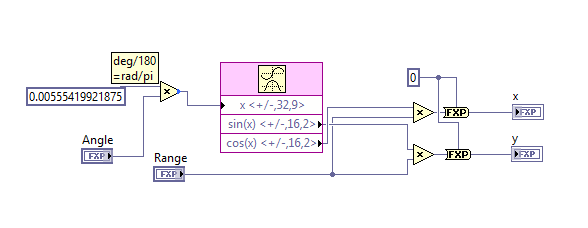
\includegraphics[scale=0.9]{Photos/pol2cart.png}
\caption{Block diagram for the polar to cartesian transformer VI}
\label{fig:pol2cart}
\end{figure}

\noindent As can be seen in Figure \ref{fig:pol2cart}, the polar to cartesian transform is a standard implementation of how one would convert an angle and distance to an X and Y coordinate. For clarity, the following diagram demonstrates how this transform is done:

\newpage

\begin{figure}[h!]
\centering
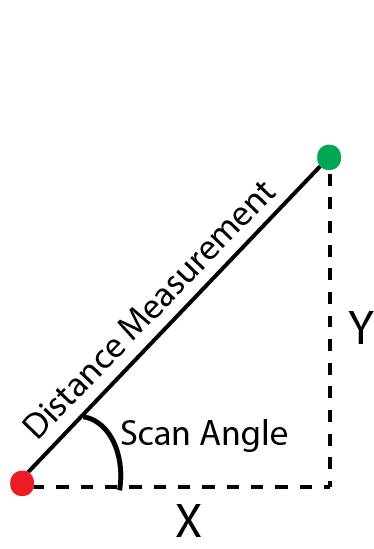
\includegraphics[scale=0.3]{Photos/pol2cart_diag.png}
\caption{Diagram of the polar to cartesian transform}
\label{fig:pol2cart_diag}
\end{figure}

\noindent As per the diagram in Figure \ref{fig:pol2cart_diag}, the polar coordinates are transformed to cartesian coordinates usign simple trigonometry: The X coordinate is obtained by multiplying the distance measurement by cos(scan angle). The Y coordinate is obtained by multiplying the distance measurement by sin(scan angle). These calculations are exactly what are shown in the block diagram in Figure \ref{fig:pol2cart}.\\ \\
%
Returning to Figure \ref{fig:transformvi}, after the polar to cartesian conversion,
%
The block diagram of the VI performing the rotation transformation of the LiDAR measurements from the LiDAR local coordinates to the vehicle coordinates is shown in the figure below:

\newpage

\begin{figure}[h!]
\centering
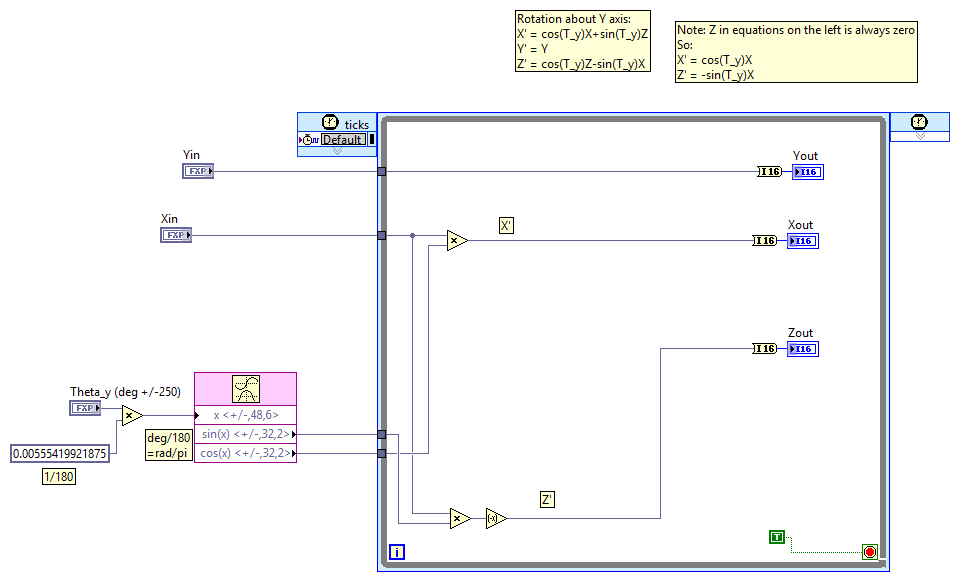
\includegraphics[scale=0.6]{Photos/rotationblock.png}
\caption{Block diagram for the VI performing the rotation transform}
\label{fig:rotationblock}
\end{figure}

\noindent Referring to Figure \ref{fig:lidarrobotaxes}, to transform the LiDAR scan data from the LiDAR local coordinate frame to the robot coordinate frame, the scan data needs to be rotated by a yaw of 45 degrees and by the pitch of the tilt unit as measured by the tilt unit encoders. As described above, the yaw is accounted for in the timed loop in Figure \ref{fig:transformvi}. Therefore, the block diagram shown in Figure \ref{fig:rotationblock} accounts for the pitch of the LiDAR. The equations that perform this transform are:

\begin{equation}
X'=\cos(pitch)X + \sin(pitch)Z
\label{eq:Xrot}
\end{equation}
\begin{equation}
Y'=Y
\label{eq:Yrot}
\end{equation}
\begin{equation}
Z'=\cos(pitch)Z - sin(pitch)X
\label{eq:Zrot}
\end{equation}

\noindent where X, Y  and Z are the scan data coordinates before the transform (i.e. coordinates in the LiDAR coordinate frame) and X', Y' and Z' are scan data coordinates after the transform (i.e. coordinates in the LiDAR coordinate frame). See this website for more details on rotation transforms and rotation matrices: \url{http://mathworld.wolfram.com/RotationMatrix.html}. \\ \\
%
In the LiDAR coordinate frame, the Z height of the points is all zero since the LiDAR performs a planar scan. So, all the Z values are zero in Equations \ref{eq:Xrot} and \ref{eq:Zrot} are zero. Therefore, Equations \ref{eq:Xrot}, \ref{eq:Yrot} and \ref{eq:Zrot} reduce to:

\begin{equation}
X'=\cos(pitch)X
\label{eq:Xrot_simplified}
\end{equation}
\begin{equation}
Y'=Y
\label{eq:Yrot_simplified}
\end{equation}
\begin{equation}
Z'=- sin(pitch)X
\label{eq:Zrot_simplified}
\end{equation}

\noindent Equations \ref{eq:Xrot_simplified}, \ref{eq:Yrot_simplified} and \ref{eq:Zrot_simplified} are what is implemented in the block diagram shown in Figure \ref{fig:rotationblock}.\\ \\
%
Finally, referring back to Figure \ref{fig:transformvi}, the last part is the translate part highlighted in the figure. As shown in Figure \ref{fig:lidarrobotaxes}, to align the LiDAR and robot coordinate frames, there is a fixed X, Y and Z distance(also known as the X, Y and Z offsets) that separates the two coordinate frames. To transform the LiDAR scan data from the LiDAR coordinate frame to the robot coordinate frame, we essentially need to account for those fixed distances. As such, the 3 addition blocks in the translate part of Figure \ref{fig:transformvi} essentially add the X, Y and Z offsets to the X, Y and Z coordinates respectively that were output from the rotation VI. Therefore, the final result is the LiDAR data, properly transformed from the LiDAR coordinate frame to the vehicle LiDAR coordinate frame.

\subsubsection{Send LiDAR Point to PC}
Referring back to Figure \ref{fig:parseandsend}, after the VI that transforms the LiDAR scan data, the last step is to send that LiDAR scan data up to the real-time code. The block diagram for the parse transform and send VI is shown below:

\newpage

\begin{figure}[h!]
\centering
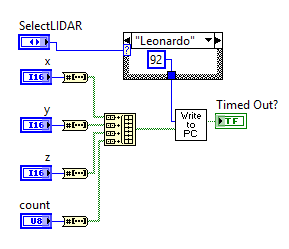
\includegraphics[scale=0.75]{Photos/inttobool.png}
\caption{Block diagram for the Parse Transform and Send VI}
\label{fig:inttobool}
\end{figure}

\noindent As can be seen in Figure \ref{fig:inttobool}, the VI takes the X, Y and Z coordinates of each LiDAR scan data point and the count which is the scan number (i.e. the nth point in the scan) for the point. The VI also takes the LiDAR that performed the scan coded as either 91 (right LiDAR) or 92 (left LiDAR). Using the number to boolean block, each integer number for X, Y, Z and count is converted to a boolean array. This is essentially converting each number into the bit definition for each number. The four boolean arrays are then concatenated together to form one long boolean array which is then passed to the write to PC VI to send to the real-time code.\\ \\
%
The block diagram for the Write to PC VI is shown below:

\begin{figure}[h!]
\centering
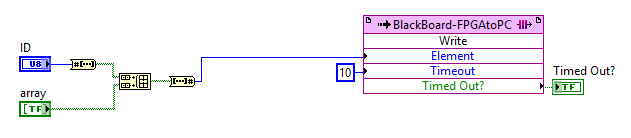
\includegraphics[scale=0.7]{Photos/sendtopc.png}
\caption{Block diagram for the Write to PC VI}
\label{fig:sendtopc}
\end{figure}

\noindent As can be seen in Figure \ref{fig:sendtopc}, the boolean array created from the integers in the Transform and Send VI is now combined with the LiDAR ID, which is also converted to a boolean array. The combined boolean array is then passed to a DMA FIFO queue that sends the data up to the real-time code from the FPGA.

\subsection{Supporting Hardware Control}

Referring back to Figure \ref{fig:hindbrainblock}, the last section of the code in that block diagram is the supporting hardware control VIs. That section of the block diagram is shown here zoomed in for convenience:

\begin{figure}[h!]
\centering
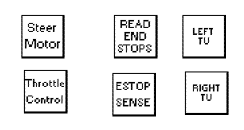
\includegraphics[scale=2.0]{Photos/supportinghardwarevis.png}
\caption{Zoomed in portion of the Hindbrain VI showing the supporting hardware VIs}
\label{fig:supportinghardwarevis}
\end{figure}

\noindent As can be seen in Figure \ref{fig:supportinghardwarevis}, there are 6 supporting hardware VIs:

\begin{enumerate}
\item Steer Motor: Controls the steering motor
\item Throttle Control: Controls the throttle and brakes
\item Rear End Stops: Senses the steering end stops
\item EStop Sense: Senses if the emergency stop switches on the vehicle (both the one in the cab and the one on the electronics box) have been depressed
\item Left TU: Controls the right tilt unit
\item Right TU: Controls the left tilt unit
\end{enumerate}

\newpage

\subsubsection{Steering Motor Control}

The block diagram for the steering motor controller is shown below:
\begin{figure}[h!]
\centering
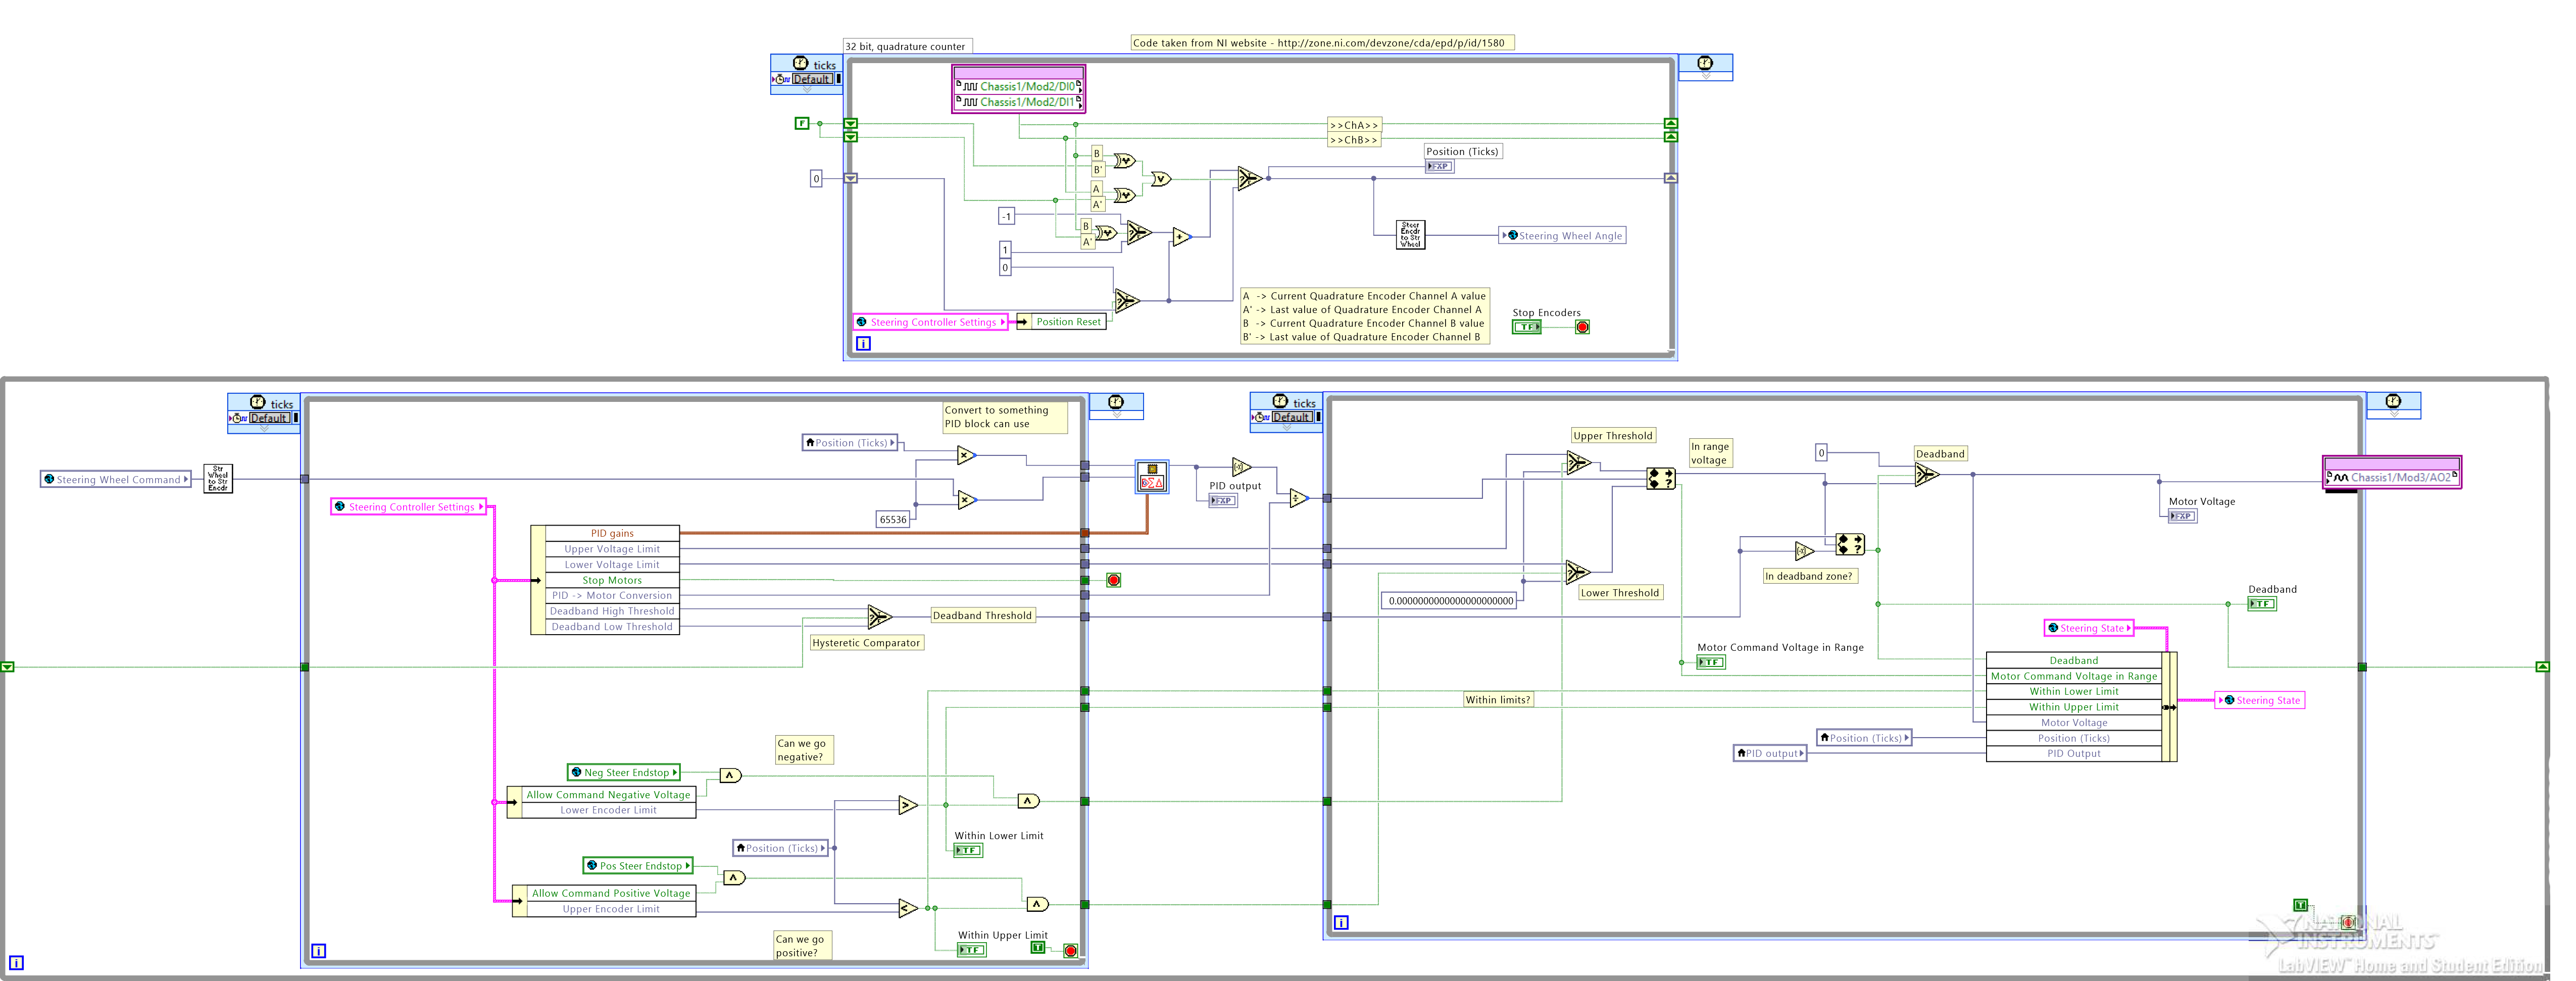
\includegraphics[scale=0.3]{Photos/steermotorblock.png}
\caption{Block Diagram of the Steering Motor Controller VI}
\label{fig:steermotorblock}
\end{figure}

\noindent The block diagram shown in Figure \ref{fig:steermotorblock} is obtained from \url{http://zone.ni.com/devzone/cda/epd/p/id/1580}. As such, this report will not discuss every aspect of the code in detail but will isntead provide a general overview. \\ \\
%
As can seen in Figure \ref{fig:steermotorblock}, there are 4 parts to the block diagram:

\begin{enumerate}
\item The upper timed while loop simply reads the quadrature encoder ticks and keeps track of the position of the steer motor based on the number of encoder ticks. That position is then converted to steering wheel angle in degrees
\item The lower left timed while loop does several things:
\begin{enumerate}
\item Converted the steering wheel angle command to encoder ticks setpoint
\item Disseminates the steering controller settings to the appropriate parts in the code
\end{enumerate}
\item A PID block that takes in the desired setpoint, PID settings and the limit and produces an output
\item Finally, the lower right timed while loop simply checks the output from the PID block to make sure it is within the set lower and upper thresholds and is not within the deadband. 
\end{enumerate}

\noindent For the PID block, it is worth noting that the inputs and outputs to the PID block are required to all be a fixed-point number with a 16-bit word length, 32-bit integer length number. This means that the inputs and outputs to the PID block must all be integer multiples of 65536 (i.e. $2^{16}$). For this reason, the inputs are multiplied by 65536 and the outputs are divided by 65536.

\subsubsection{Throttle Control}

The block diagram for the VI that controls the gas and brake pedal is shown below:

\begin{figure}[h!]
\centering
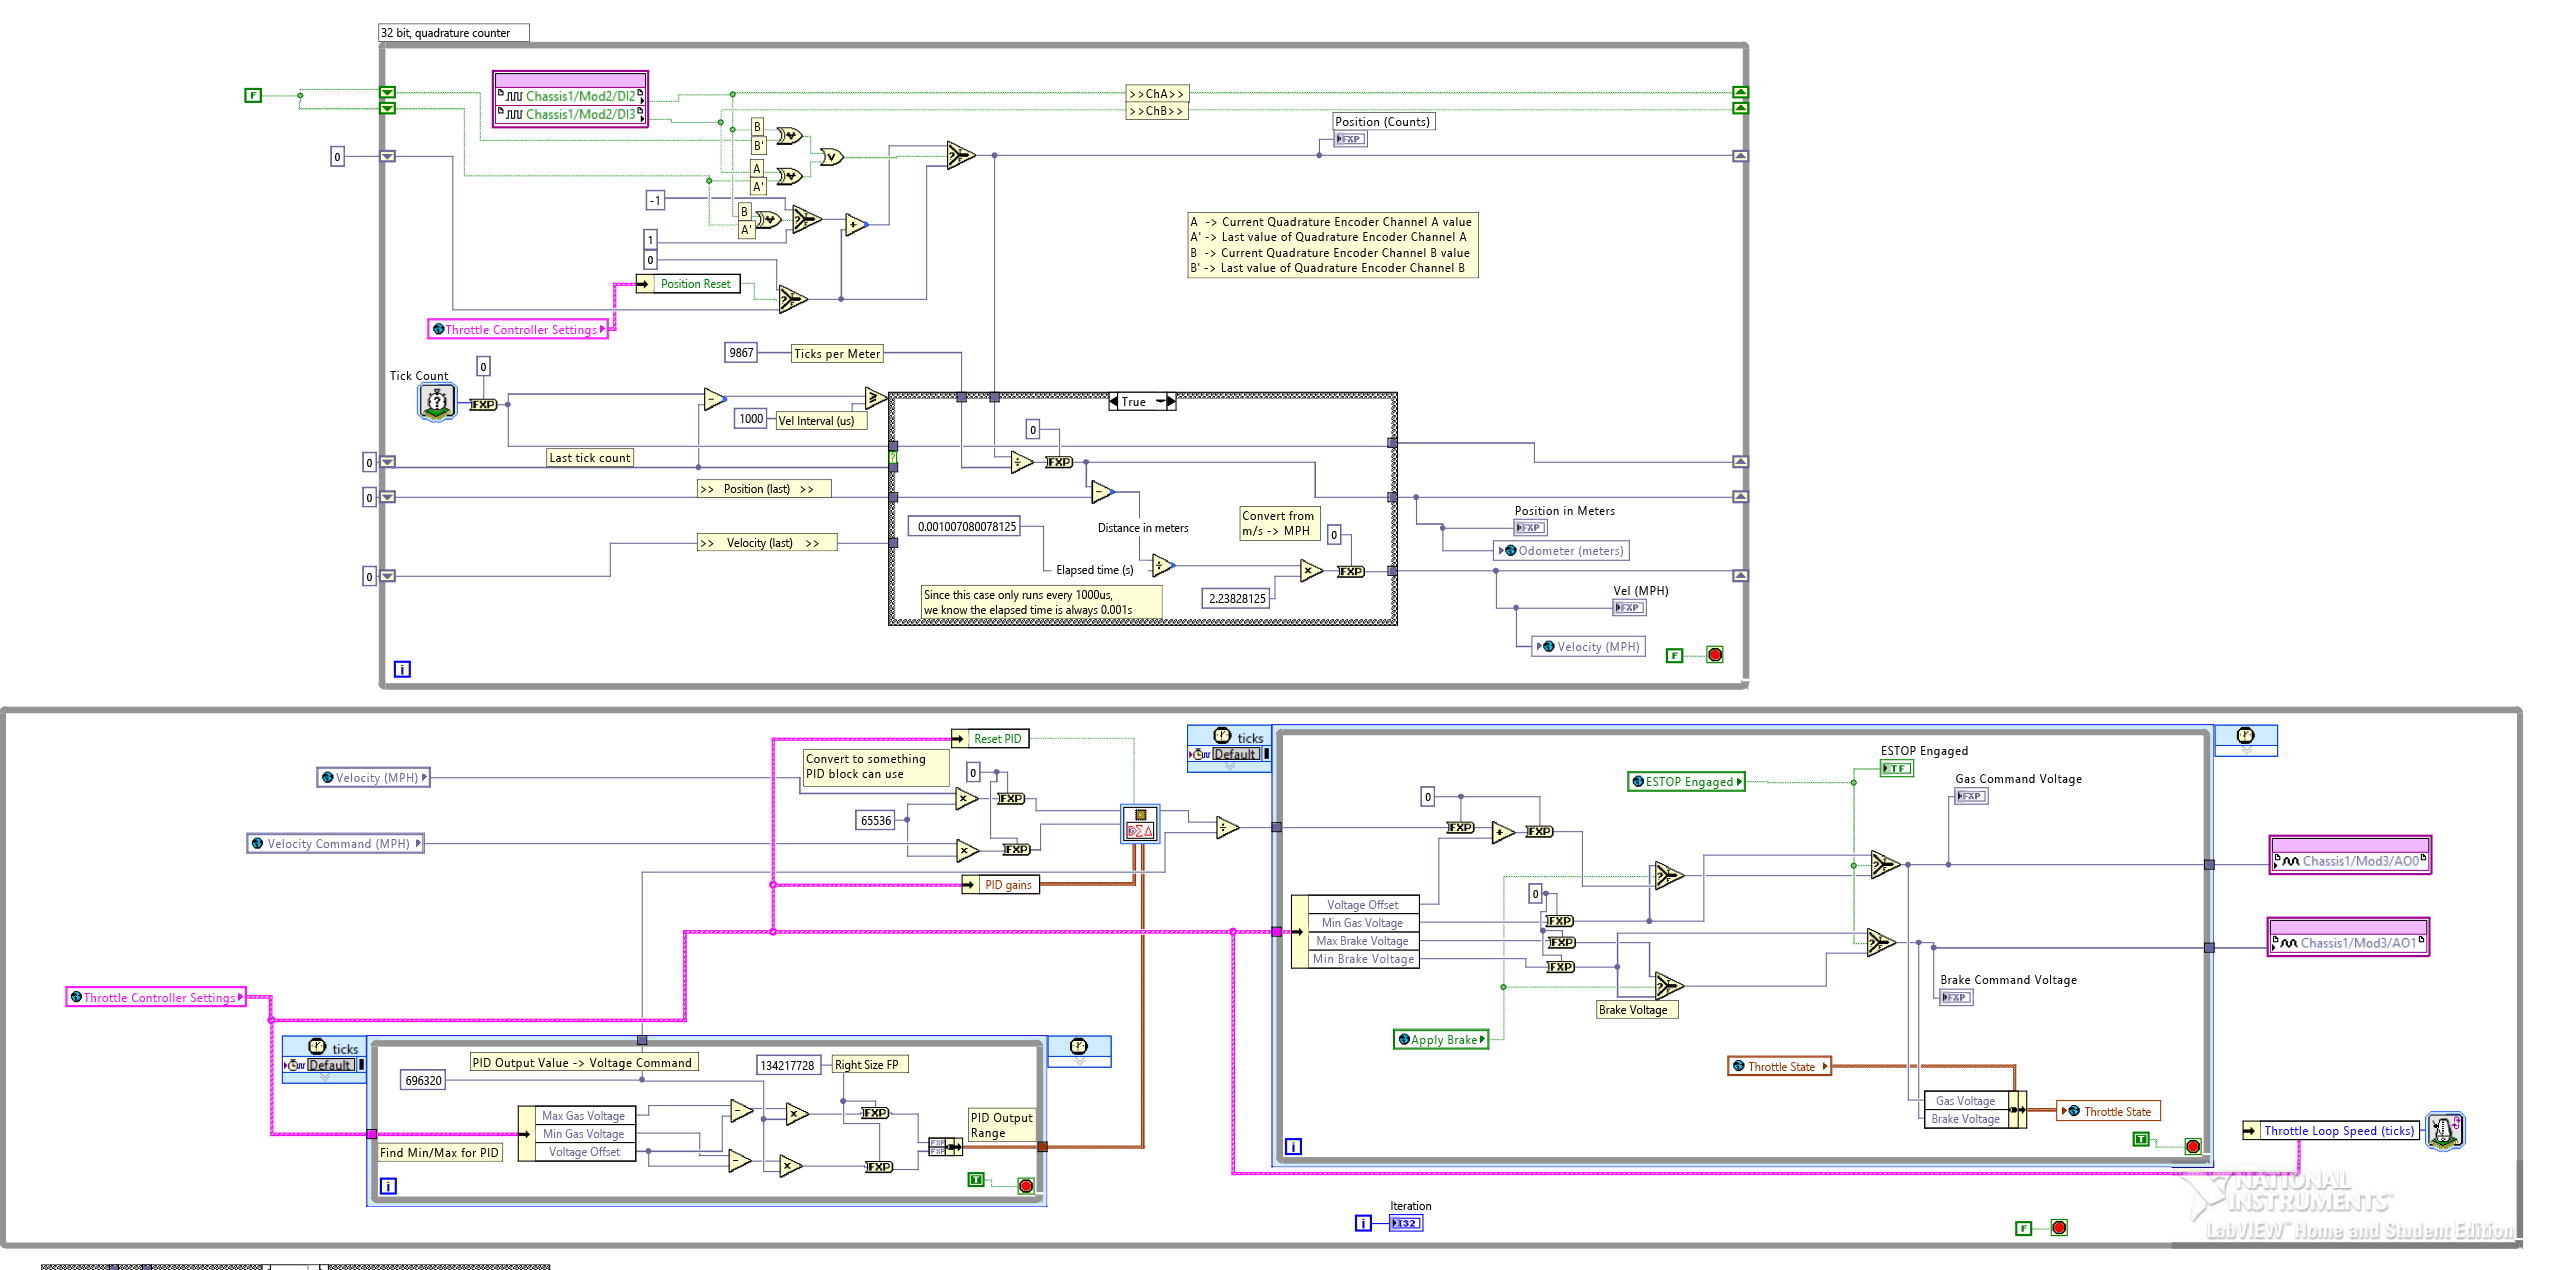
\includegraphics[scale=0.75]{Photos/throttlecontrol.png}
\caption{Block Diagram of the Throttle Control VI}
\label{fig:throttlecontrol}
\end{figure}

\noindent As shown in Figure \ref{fig:throttlecontrol}, there are two main while loops:

\begin{enumerate}
\item The upper while loop simply monitors the quadrature encoder on the rear wheels and computes the velocity and distance traveled by the vehicle. 
\item The lower while loop then controls the gas pedal based on the speed of vehicle calculated in the upper while loop. The PID block in that while loop therefore controls the vehicle speed by comparing the calculated vehicle speed and the desired vehicle speed and produces an output that is used to control the gas pedal. 
\end{enumerate}

\noindent Also note that at the bottom of the bottom right timed while loop in Figure \ref{fig:throttlecontrol}, the loop also takes a boolean that represents whether the brakes need to be activated or not. The loop then controls the brake pedal to apply the brake when the boolean is true.

\subsubsection{Read End Stops}

The VI that reads the end stop sensors is simple and is shown in the figure below:

\begin{figure}[h!]
\centering
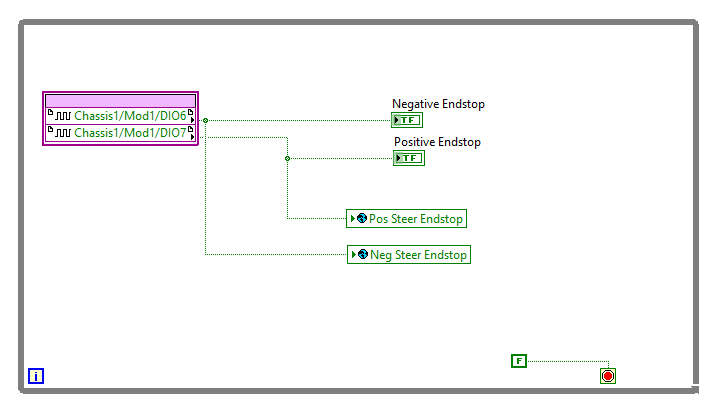
\includegraphics[scale=0.75]{Photos/ReadEndStops.png}
\caption{Block Diagram of the Read End Stops VI}
\label{fig:readendstops}
\end{figure}

\noindent The VI simply reads the state of two digital pins, 1 for each end stop (cherry) sensor, and writes the boolean balue to the appropriate FPGA global variable. 

\newpage

\subsubsection{EStop Sense}

The block diagram for the VI that sense the activation of the emergency stop buttons on the vehicle is shown below:

\begin{figure}[h!]
\centering
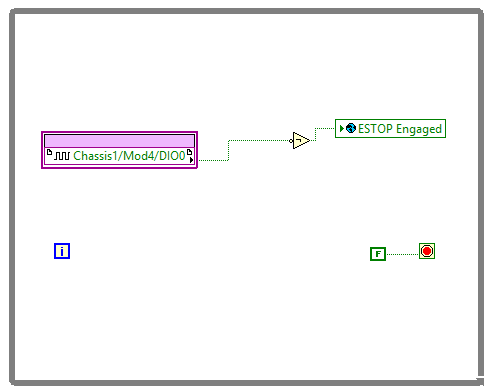
\includegraphics[scale=0.75]{Photos/estopsense.png}
\caption{Block Diagram of Emergency Stop Sense VI}
\label{fig:estopsense}
\end{figure}

\noindent Like the Read End Stops VI, this VI also simply reads a digital pin to determine if either of the estop buttons on the vehicle have been depressed. The while loop then passes the boolean up to an FPGA gobal variable so that the real-time code can have access to that information.

\newpage

\subsubsection{Right and Left Tilt Unit Control}

The block diagram for the left and right tilt unit controllers is shown in the figure below:

\begin{figure}[h!]
\centering
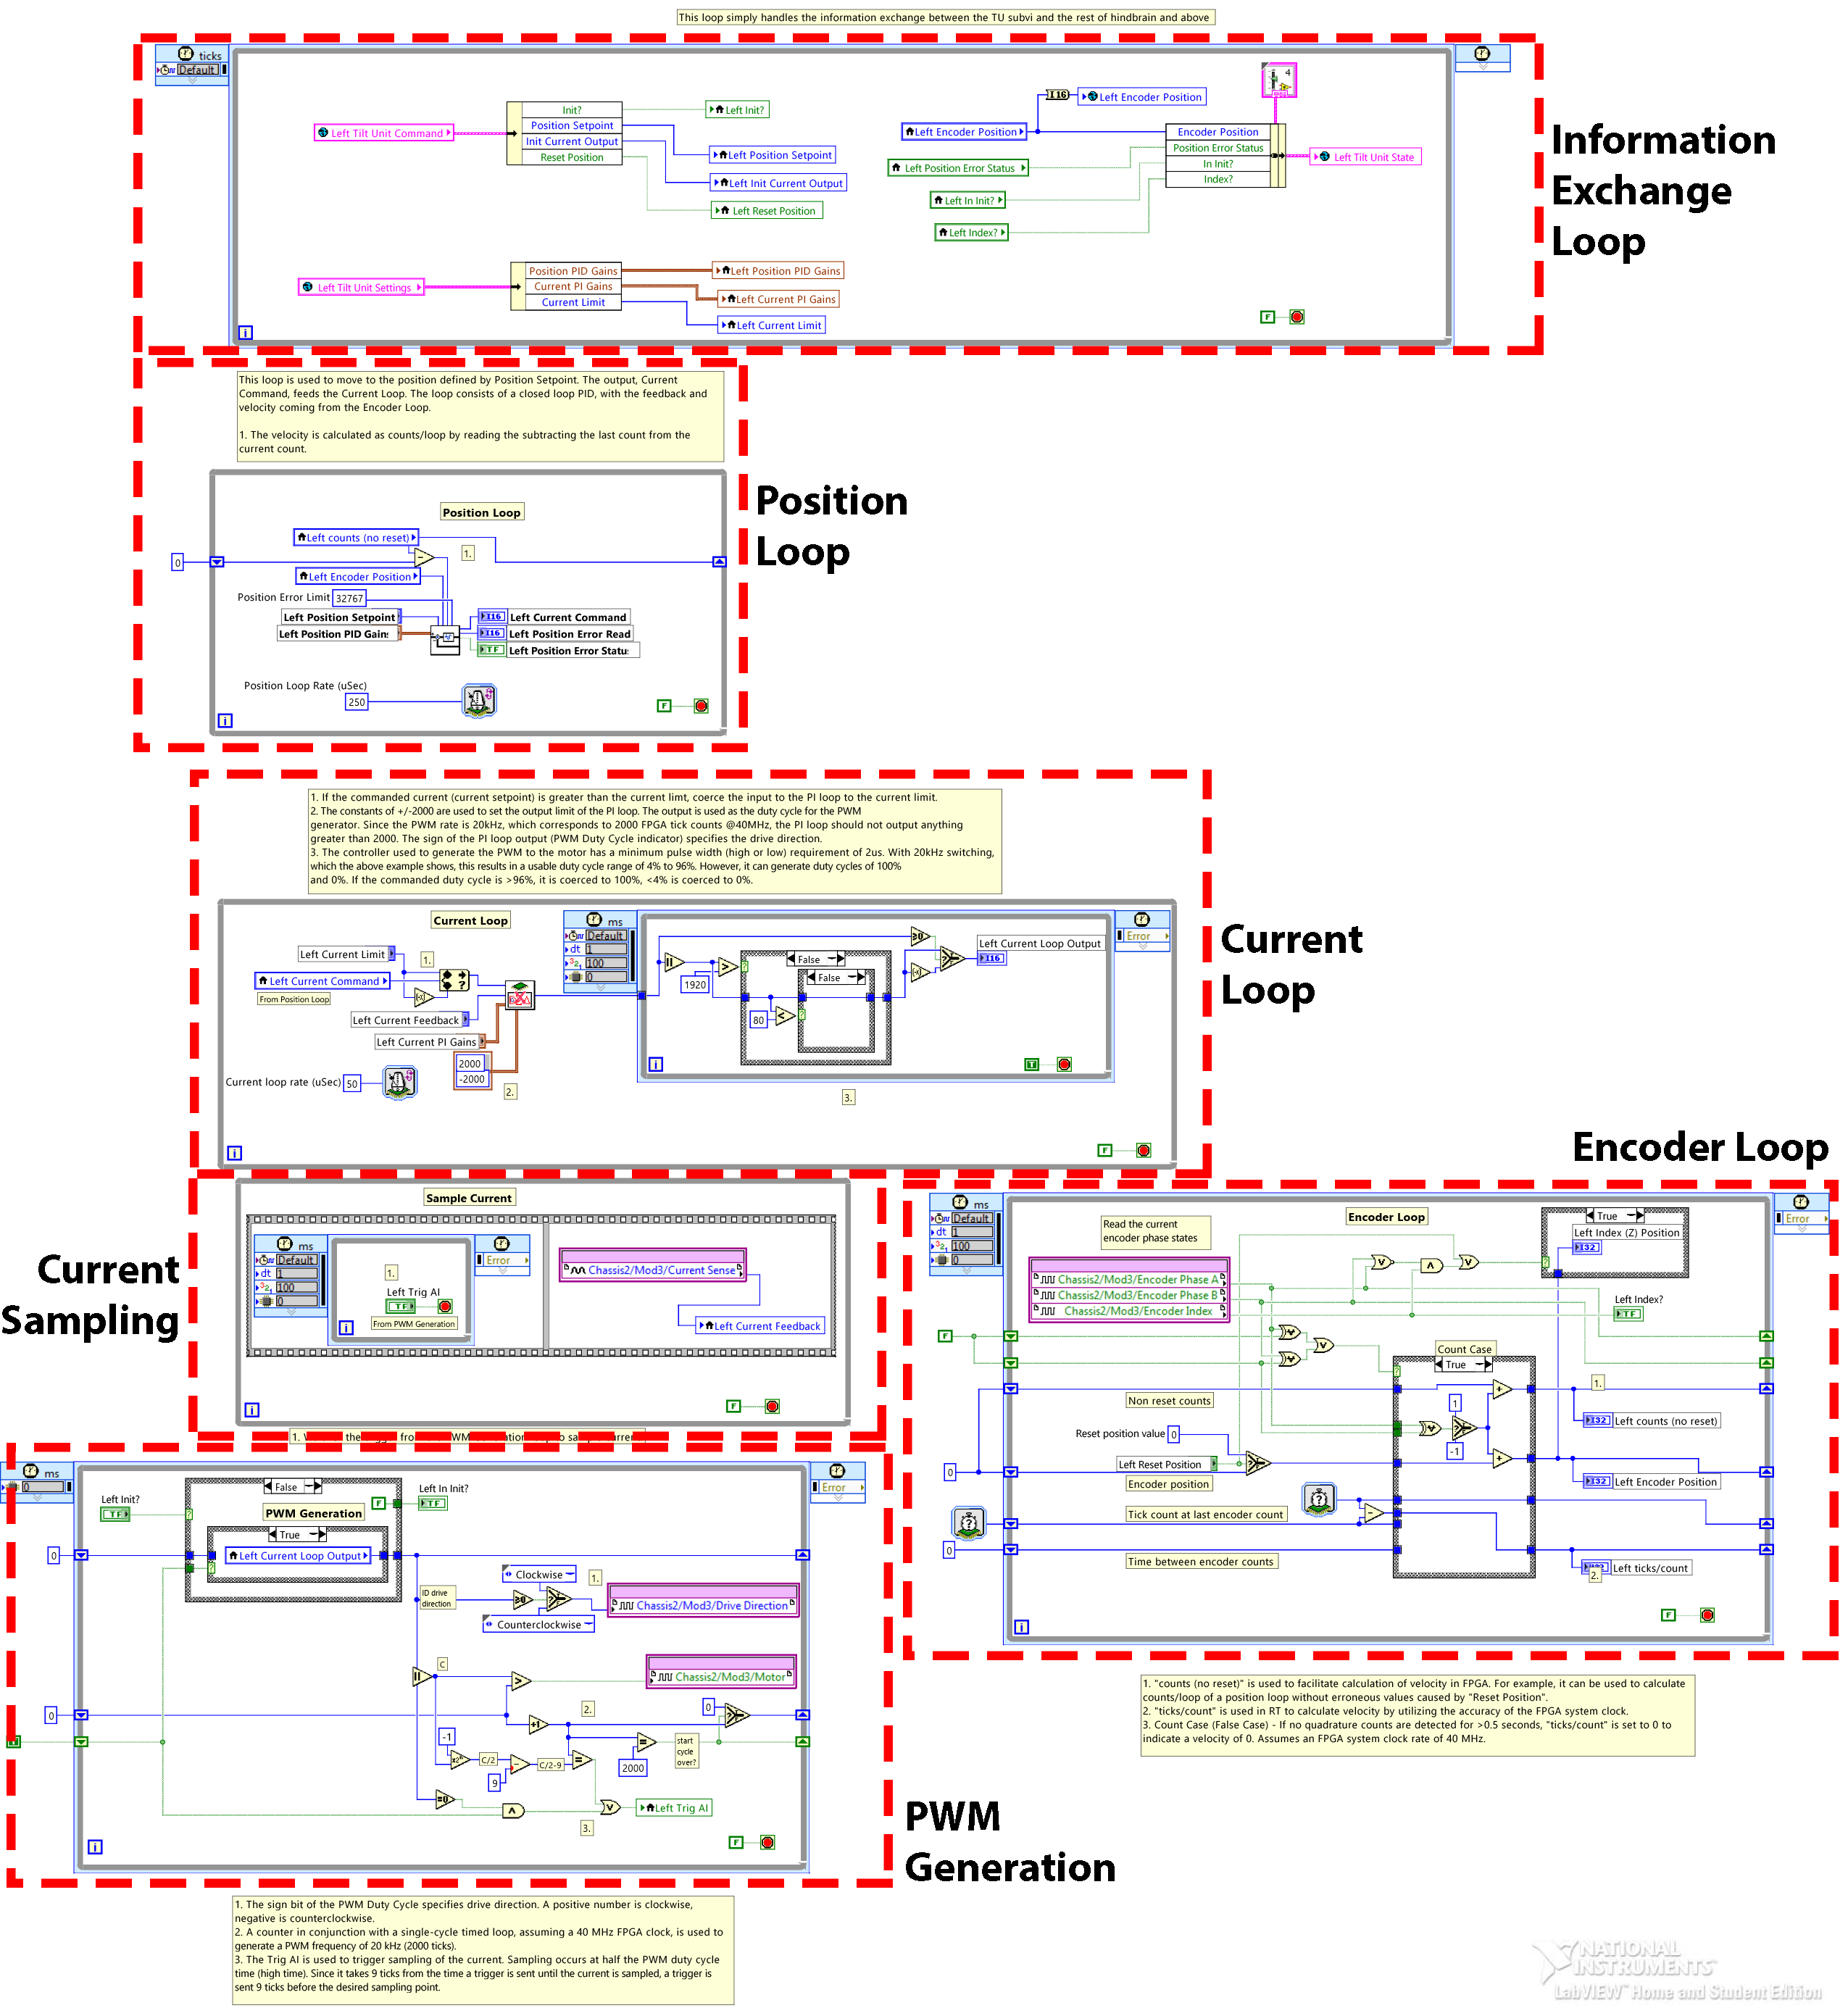
\includegraphics[scale=0.65]{Photos/tucontroller.png}
\caption{Block Diagram of the Left and Right Tilt Unit Controller}
\label{fig:tucontroller}
\end{figure}

\noindent Note that although the left and right tilt unit controllers are separate VIs as shown in Figure \ref{fig:supportinghardwarevis}, the two VIs are exactly the same except for the chassis and module number that is set on the blocks that write and read from the NI modules since the left and right tilt units are each controlled by a separate NI 9505 module.\\ \\
%
As shown in Figure \ref{fig:tucontroller}, the tilt unit controller is made up of 6 parts:

\begin{enumerate}
\item Information exchange loop: The information exchange loop is simply responsible for reading the state of the tilt unit and writing commands to the tilt unit controller code. So, for example, the tilt unit commands are received from the real-time code and, through the information exchange loop, passed down to the relevant parts of the tilt unit control code. Similarly, the tilt unit state is read from the various parts of the tilt unit control code and, through the information exchange loop, is made available to the real-time code to read.
\item Position loop: The position loop simply provides PID control over the position of the tilt unit using the PID settings specified in the tilt unit settings cluster.
\item Current loop: The current loop simply provides PI control over the current output to the tilt unit motor using the PI settings specified in the tilt unit settings cluster.
\item Current Sampling: Samples the current output to the tilt unit motor.
\item Encoder loop: Reads the quadrature encoder on the tilt unit and keeps track of the position of the tilt unit in units of encoder ticks.
\item PWM Generation: Generates the PWM signal used to drive the tilt unit motor. 
\end{enumerate}

\noindent Note that there is a case statement around the desired current used in the PWM generation loop that selects the source of the desired current. Also note that there is a 'Init?' switch that allows the real-time code to switch the mode of the tilt unit controller to either be in init mode or normal running mode. \\ \\
%
The tilt unit controller code was designed to operate in the following way:

\begin{enumerate}
\item If the tilt unit is running in normal running mode (i.e. the 'Init?' switch is set to false), the six loops essentially carry out standard torque control to maintain the tilt unit at a desired setpoitn position. In this case, in the PWM generation loop, the source of the desired current is the current put out by the current loop.
\item If the tilt unit is running in initialize mode, the source of the desired current in the PWM generation loop is simply the desired initialize current set in the real-time code. In this case, the control output from the six loops is ignored and the PWM generation loop is simply given a fixed desired current to operate in during initialization.
\end{enumerate}

\subsection{Relay Control}

The last part of the Hindbrain VI shown in Figure \ref{fig:hindbrainblock} is the relay control. For convenience, the relay control portion of the block diagram is zoomed in and shown below:

\begin{figure}[h!]
\centering
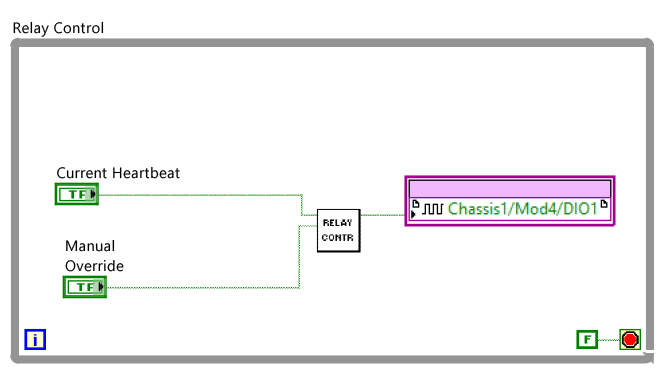
\includegraphics[scale=1.4]{Photos/relaycontrolportion.png}
\caption{Block diagram of the relay control of portion of the hindbrain}
\label{fig:relaycontrolportion}
\end{figure}

\noindent This relay controller serves as a key safety system for the vehicle and the while loop allows LabVIEW to trigger the emergency stop system and will only allow the vehicle's autonomous systems to stay active only if all levels of control code (i.e. FPGA, LabVIEW midbrain, ROS midbrain and ROS forebrain as well as OCU code and remote emergency stop) must be running and active. If any of the code freezes or execution is suspended, LabVIEW should trigger the emergency stop. As such, as shown in Figure \ref{fig:relaycontrolportion}, the while loop  takes as input the heartbeat the represents proper running of all other layers of code from the real-time code and also a manual override that is included to allow a human operator to override the decisions of the autonomous code to control the relay. This is then fed into a subVI that determines if the heartbeat boolean is running as expected and the output of that subVI controls the state of the relay. \\ \\
%
The block diagram for that subVI is then shown in the figure below:

\begin{figure}[h!]
\centering
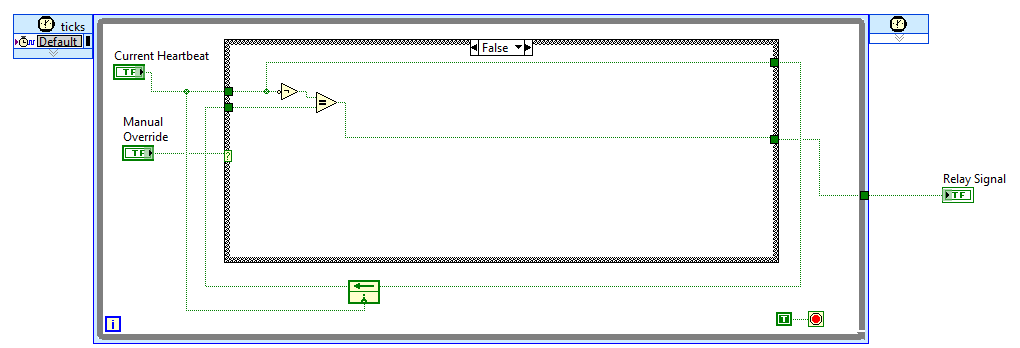
\includegraphics[scale=0.55]{Photos/relaycontrolsubvi.png}
\caption{Block diagram of the relay control subVI}
\label{fig:relaycontrolsubvi}
\end{figure}

\noindent As can be seen in Figure \ref{fig:relaycontrolsubvi}, the subVI essentially checks to see that the heartbeat is alternating between true and false each cycle through the loop. If this alternating behavior of the heartbeat is not observed, the VI will trigger the emergency stop system and shut the robot down.\\ \\
%
It must be noted at this point that although the code is designed to operate in this way, the hardware is not ready to support this. Specifically, there needs to be a hardware adapter that allows the FPGA digital I/O module (that can only source 1mA of current) to operate a relay that typically has a higher current draw than 1mA. A future team will need to adjust the relay hardware to make this relay system function in this way. 
\newpage
\chapter{The Robot Software System (ROS)}

The ROS system is designed to contain as few customizations as possible. This allows our team and future teams to take advantage of as many pre-existing ROS packages as possible. Note that this section of the report assumes familiarity with ROS, basic ROS functionality, catkin and how to create and use ROS packages.

\section{Overview of the Packages}
The ROS software stack of the vehicle contains the following catkin packages: 

\begin{enumerate}
\item gator\textunderscore odom: Contains a script and launch file that generates the wheel odometry information
\item gator\textunderscore nav: Contains the launch and yaml files that are required to set the settings for the navigation stacks and launch the navigation stack
\item gator\textunderscore msgs: Defines any custom messages that are created specifically for the Gator
\item gator\textunderscore localization: Contains the launch files needed to launch the necessary robot\textunderscore localization and navsat\textunderscore transform nodes to allow the Gator to localize accurately
\item gator\textunderscore description: Contains the launch files, STL files and URDF file that create a visual model of the Gator
\item gator\textunderscore communication: Contains python scripts that listen to all sensor data coming from LabVIEW over UDP and publishes it in ROS to the appropriately named topic
\item gator: An unused package that was set up for the purpose of containing all the highest-level launch files for running the vehicle
\end{enumerate}

\section{Preparing to Run the ROS Stack and Setting up the Repository}

The NUC onboard the Gator already has all the packages required to run the software stack in ROS Indigo. However, if you want to run the software stack on another computer, you should try to sta with ROS Indigo unless the IV Lab has upgraded its fleet. You'll then need the following ROS packages to be isntalled using apt-get and the standard style of installing ROS packages (e.g. sudo apt-get install robot-localization-indigo):

\begin{enumerate}
\item Robot Localization: \url{http://wiki.ros.org/robot \textunderscore localization}
\item move base: \url{http://wiki.ros.org/move \textunderscore base}
\item URDF: \url{http://wiki.ros.org/urdf}
\end{enumerate}

\noindent Once these packages are installed, you can then download the Gator repository from here: \url{https://github.com/olinrobotics/GatorResearch}. Once downloaded, change directory into the master \textunderscore ws folder and then run the command "catkin \textunderscore make". Once done, run the command "source devel/setup.bash". If desired, you should add this sourcing step to your bashrc file so that you don't have to do this manually every time you open a new terminal.

\newpage

\section{ROS Navigation Overview}

The following diagram shows how the ROS Navigation Stack is designed to be used:

\begin{figure}[h!]
\centering
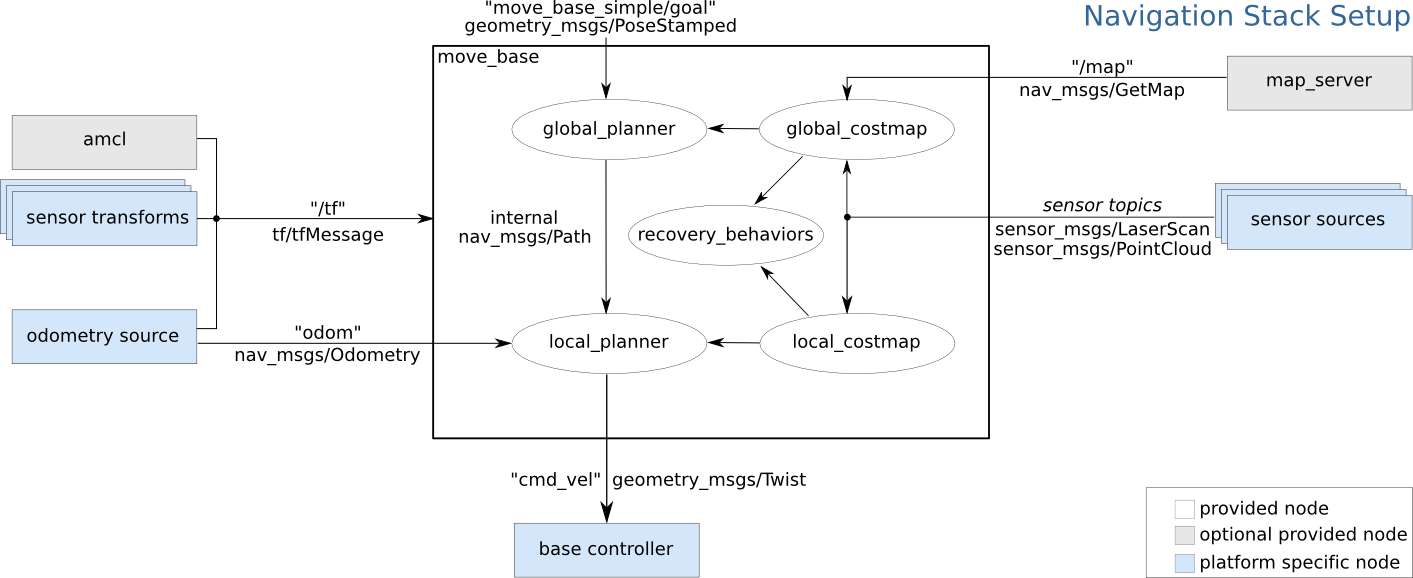
\includegraphics[scale=.35]{Photos/rosnavoverview.png}
\caption{Overview of the Setup of the ROS Navigation Stack}
\label{fig:rosnavoverview}
\end{figure} 

\section{gator\textunderscore odom}

The gator\textunderscore odom package contains the following files:

\begin{enumerate}
\item wheel\textunderscore odom.py: Creates a wheel odometry node that reads the odometry calculations made by LabVIEW and uses that odometry information to compute the odometry transform from the origin of the vehicle (i.e. on the ground under the rear axle of the vehicle) to a fixed-frame coordinate system called odom. 
\end{enumerate}

\newpage
\chapter{The OCU Software System}

%\begin{figure}[h!]
%\centering
%\includegraphics[scale=.08]{wholefish.jpg}
%\caption{The current version of the robotic tuna}
%\label{fig:wholefish}
%\end{figure} 


\end{document}
